\chapter[ASTHROS Payload Readout System Design]{ASTHROS Payload Readout System Design}
\label{ch:readout}
ASTHROS, the Astrophysics Stratospheric Telescope for High Spectral Resolution Observations at Submillimeter-wavelengths, is a balloon-borne observatory designed to study the universe in the submillimeter wavelength range.
This chapter describes the design and implementation of the ASTHROS payload readout system, which is responsible for controlling the detectors, reading out the data, and storing the data on a solid state drive.
Additionally, the readout system is responsible for communicating with the gondola system which sends commands to the payload and receives data from the payload to send to the ground control system.
In addition to reading out from our detectors, the readout system communicates with other hardware on the payload, such as the power supply units and antenna systems, to monitor their status and control their operation.
The readout system is designed to be modular and scalable, allowing for easy integration of new detectors and readout systems.
Each package is designed to be self-contained, focusing on a single device in the readout system, so that changes to the hardware can be made without affecting the rest of the system.

The primary function of this chapter is to describe the readout system in excruciating detail so future users can understand how every part of ASTHROS works as well as the design decisions made during the development of the system.
While this is not a traditional chapter in the dissertation sense, it is an important part of the work done during my research and documenting the system is vital to the success of the project.
Without developing a readout system, my on-board autonomy work in Chapter \ref{ch:spectra} would have nowhere to run and no data to process.

\section{Introduction}
The ASTHROS payload readout system is a fully modular network of subsystems that communicate with each other over a RabbitMQ network.
Each piece of hardware on the payload had custom drivers developed to wrap the native interface of the hardware in a common structure so all devices on the network can communicate with each other with a common protocol.
At the trade off of a more complexity during initial development, this design allows for easier integration of new devices and subsystems into the readout network.

This chapter is divided into several sections that describe the design and implementation of the readout system.
The network architecture of the readout system is described first, including the devices and subsystems that make up the network.
Details are provided about the processes running on each device and how they communicate with each other.
For the Raspberry Pi Compute Module 4, the process of setting up the device to run the readout system is detailed, including the necessary packages and libraries that need to be installed, as this system is often used in a standalone setting with the \texttt{PyMCC} package.

Next we will describe the RabbitMQ message broker that is used to communicate between the devices on the readout network.
This section will give an overview of how RabbitMQ works and how it is used in the ASTHROS readout system.
Following that, we describe the functionality of the \texttt{RMQTools} package that we developed to simplify the process of creating publishers and subscribers to the RabbitMQ network.
This package is used in every device on the readout network to communicate with the RabbitMQ server and send messages and receive commands.

Following that, we go into detail about the modules developed to run subsystems on the readout network.
For our science data, we detail the Pacific MicroCHIP Corporation (PMC) P19800B ASIC RF Spectrometer, or PMCC, which is the primary detector used on the ASTHROS payload and the \texttt{PyMCC} package that was developed to control the PMCCs and read out the data.
Following that, we describe our Cryocool control system used to control the cryocooler that cools our detectors.
Next, we describe the Antenna controls that are used to monitor the antenna temperature and control the secondary hexapod. 
After that, we describe the Motor controls that are used to control a small stepper motor that we use to chop between the sky and a blackbody reference.
All of these systems are controlled by a custom built Power Supply Unit (PSU) whose functionality we wrapped to allow us to control over the network.
And finally, we describe the Variable Attenuators in both their hardware design and the firmware used to control them.

Following all of this, we describe two of the harmonizing modules that are used in the ASTHROS readout system.
The first is Housekeeping which combines status messages from all of the previous modules and sends them to the ground control system.
The second is the Central Command module which is used to send commands to the devices on the readout network and receive responses from them.
Finally, we conclude with a summer of next steps for the system and the plan for integration of Chapter \ref{ch:spectra} with the readout system on the Analysis computer. 

\section{Network Architecture}
\begin{figure}
    \centering
    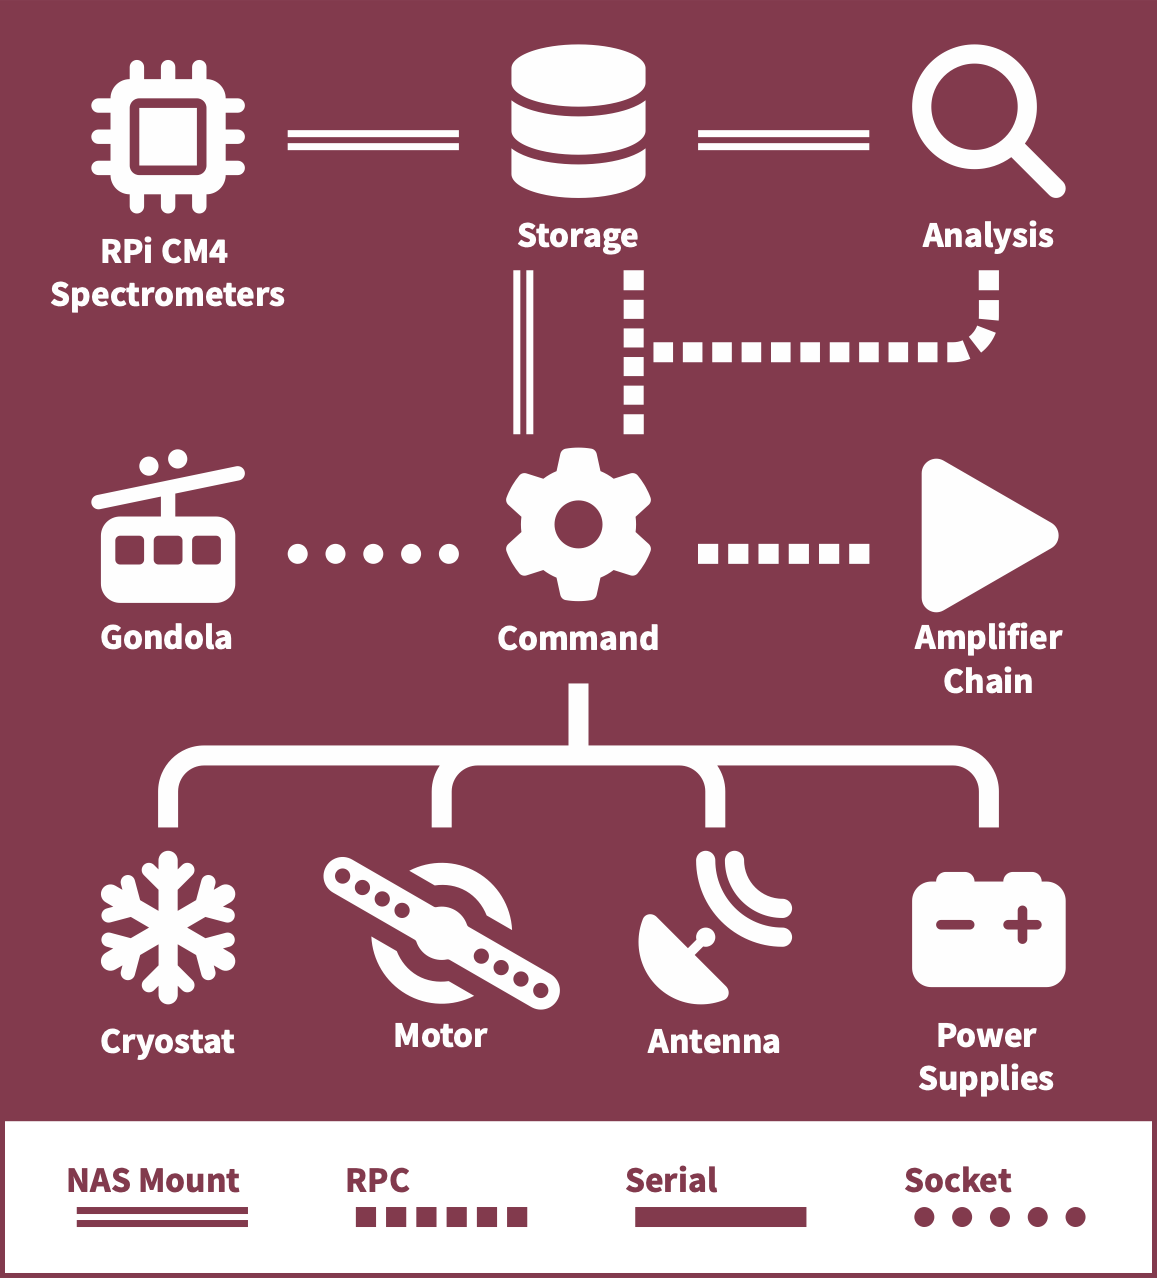
\includegraphics[width=0.5\linewidth]{figs/spectra/system.png}
    \caption[High Level System Diagram for ASTHROS]{A high level overview of the ASTHROS Readout Network System Architecture showing the Command, Storage, and Analysis computers. The Command computer is responsible for sending commands to other processes and receiving status updates from the various publishers on the RMQ network. The Storage computer is responsible for storing all science data and telemetry data collected during the flight. The Analysis computer is responsible for analyzing the science data collected during the flight. The overview also shows some of the various subsystems and how they're connected in the network.}
    \label{readout/fig:system}
\end{figure}

On board, we have four main types of devices that make up the readout network.
Figure \ref{readout/fig:system} shows a high level overview of the readout network architecture.
The first is the command computer, a WinSystems fight computer, which is our primary command and control computer.
It is physically connected to the power supplies, antenna, cryocooler systems, and the motor controls for the chopper.
Each of these systems is a custom process run on the command computer and they communicate with each other over the RabbitMQ network.
Additionally, the command computer is responsible for running the Housekeeping and Central Command modules that are used to send commands to the devices on the readout network and receive status updates from them.
The command computer connects to the rest of the system via a wired Ethernet connection to our Storage computer's network switch.

The second type of device is the storage computer, a custom RTD Embedded Technologies PC/104 stack.
The PC/104 form factor is a standard for embedded computers that allows for stacking of multiple boards to create a custom computer system \parencite{5731130}.
In our configuration, the PC/104 stack consists of a main compute board, two managed network switches, three bays for solid state drives, and a power supply board.
This gives our Storage computer the ability to connect up to 16 devices to the readout network. 
As this computer is centrally located on the network, it hosts the RabbitMQ server that is responsible for routing messages between all the devices. 
Like the name implies, the Storage computer is responsible for storing all of the science and housekeeping data collected during the flight.
We utilize four 4TB solid state drives in either a RAID 5 or 10 configuration to provide a total of 12 or 8 TB of storage for the science data.
The decision between RAID 5 and 10 is based on the our level of redundancy and storage requirements. 
With RAID 10, we have a total of 8 TB of storage, but we can survive at least a single drive failure without losing any data.
With RAID 5, we would have more storage at 12 TB but would only be able to survive one drive failure.
Currently, we use a RAID 10 configuration but would be open to switching to RAID 5 if we need more storage in the future after recalculating our data rates. 

The Storage computer is configured as a Network Attached Storage (NAS) device that allows other computers on the network to access the data.
This allows systems to mount the NAS and save data directly to the NAS without having to worry about the underlying storage system.
In addition to science data, the Storage computer is also responsible for storing all of the telemetry data collected during the flight.
As a proof of concept, we've developed an ODOO sever that uses a PostgreSQL database to store housekeeping. 
The ODOO server allows for web-based access to the data for real time monitoring of the payload.
This is useful in test configurations when we have easy access networking to ASTHROS and can load the ODOO web application on connected devices.
ODOO has workers that are configured as subscribers to the RabbitMQ network and will receive messages from various sources and route them to the correct database tables.

The third system is the Analysis computer, an NVIDIA Jetson based system that is responsible for analyzing the science data collected during the flight.
The Analysis computer is connected to the Storage computer via a wired Ethernet connection and is responsible for running the on-board autonomy system that processes the science data and sends it to the ground control system.
Currently, the Analysis computer is our least developed system as we are still working on integrating the on-board autonomy system with the readout network.
The final system will mount the NAS and connect to the ODOO server to review a queue of science data that needs to be processed.
Details for implementation of the on-board autonomy system are described later in Section \ref{readout/section:future}.

Finally, we have the Raspberry Pi Compute Module 4s (CM4s) that are used to control the PMCCs. 
Each CM4 is physically connected to up to four PMCCs via SPI and is responsible for reading out the data from the PMCCs and saving it to the Storage computer through the NAS mount.
We do not send our raw data through the RabbitMQ network in order to reduce the load on the system for non control critical data. 
The CM4s are connected to the Storage computer via a wired Ethernet connection and communicate with the RabbitMQ server to send status updates and receive commands.
These CM4s are often used in the lab independently of the rest of the readout network.
As such, we have included a guide on how to setup a CM4 in Appendix \ref{readout/app:cm4_setup}.

\section{RabbitMQ}
\label{readout/section:rmqtools}
The ASTHROS readout system relies on RabbitMQ to communicate between different devices and systems on the readout network.
Past ballooning missions, such as BLAST-TNG, utilize sockets to communicate between systems \parencite{gordon2019highly}.
The resulting network of sockets across multiple devices becomes difficult to manage and debug as many of the definitions for the sockets are hard coded into the software.
Devices in such a system often use User Datagram Protocol (UDP) to broadcast messages across the network.
This approach requires each device to listen for messages on a specific port and parse the messages to determine if they are intended for that device.
For systems that require multiple devices to communicate with each other, this can become cumbersome as each device must be aware of the other devices on the network and the ports they are listening on.
Additionally, UDP is a connectionless protocol, meaning that there is no guarantee that a message will be received by the intended recipient.
To work around this, the BLAST readout systems was built as a single monolithic program that orchestrates all the devices on the network.
This approach is not scalable and makes it difficult to debug and maintain the system.

For ASTHROS, we wanted to build a system that was modular, consisting of microservices that can easily be integrated into the rest of the system using a shared protocol.
To accomplish this, we needed to decouple the devices in a way that data production and consumption are separated.
Services that produce housekeeping data are not concerned with who needs the data, and services that consume housekeeping data are not concerned with where the data comes from, simply how the data is formatted. 
This is where a message broker like RabbitMQ comes in.
RabbitMQ is an open-source Advances Messaging Queue Protocol (AMQP) implementation that serves as a broker for incoming and outgoing messages by routing messages to bound destination queues located on an exchange \parencite{dunne2018comparison}.
We chose RabbitMQ because of the centralized message broker architecture that allows for easy integration of new devices and services.
All of our devices are networked together, making a centralized message broker the ideal solution for our readout system.

The core of RabbitMQ is explained on the documentation as well as \cite{toshev2015learning}.
We like to use a post office analogy to explain how RabbitMQ works.
Within RabbitMQ are three main components: producers, queues, and consumers. 
Producers are the senders of a message, which is analogous to a person sending a letter.
In our case a message is any binary of blob of data, but we typically use JSON formatted strings.
When a producer sends a message, it addresses the message with a routing key.
A queue is similar to a mailbox where letters are stored until they are picked up by the recipient.
The recipient of the message is the consumer, who retrieves the message from the queue.
Just like a normal mailbox, a queue can have multiple producers sending data to it and multiple consumers who can try and read the data.

In all of this, the message broker is the post office and postal workers.
When a producer makes a message, it hands it to the post office to be delivered to all who need it.
This is done using the routing key that specifies the queue the message should be delivered to.
The post office then takes the message and delivers it to the correct mailbox. 
When a consumer is ready to read a message, it checks its mailbox for any messages and reads them.
If the consumer is not ready to read the message, the message stays in the mailbox until the consumer is ready.

Behind the scenes, there is a fourth concept important to RabbitMQ: exchanges.
Exchanges are the post office's sorting facility.
Typically, producers are not typically sending messages directly to queues. 
Instead, they publish messages to an exchange with a specific routing key.
When a queue is made, it can be bound to an exchange with routing keys.
If the routing key of the messages matches one of the routing keys bound to the queue, the message is delivered to that queue.
Routing keys can be wildcards, allowing queues to subscribe to specific types of messages. 
For ASTHROS, we follow the format of \texttt{<type>.<device>.<subtype>} for our routing keys.
For example, a housekeeping value from temperature sensors on Power Supply Unit 4 would be \texttt{housekeeping.temp.4}.
This allows a queue to be bound broadly to a specific type of message, such as \texttt{housekeeping.*.*} to receive all housekeeping messages or \texttt{*.temp.*} to receive all temperature messages.
For systems that have multiple devices, this allows us to easily ingest all data from those devices without having to know the specific routing keys for each device.

\subsection{RMQTools}
While RabbitMQ serves as a powerful backbone for our networking infrastructure, we needed to develop a way to wrap our devices in ways that will communicate with the RabbitMQ server.
To accomplish this, we developed a Python package called \texttt{RMQTools} that provides a simple interface for creating both publisher to subscriber systems as well as Remote Procedure Call (RPC) frameworks.
At its core is the \texttt{RmqConnection} class that wraps the \texttt{pika} library to add additional functionality and simplify the process of creating a RabbitMQ connection \parencite{pika}.
Pika is a single threaded RabbitMQ client library in python that provides an implementation of the AMQP protocol.
Many of our modules will require threading as we will often have a main thread running processes on the hardware while a second thread is running the RabbitMQ connection making it difficult to use the \texttt{pika} library directly.
\texttt{RmqConnection} handles this threading by allowing us to create a connection to the RabbitMQ server and run the connection in a separate thread from the main thread.

As a simple example of publisher to subscriber systems, we instantiate the \texttt{RmqConnection} class as an \texttt{rmq} object with the RabbitMQ server address and port as well as the username and password for the server.
We can then use \texttt{@rmq.set\_status\_exchange(name)} to specify which status exchange we will be using. 
These are done for on both the publisher and subscriber side, ensuring that both are using the same server and exchange. 
Now that we have configured the setup, we can implement a publisher.
This is done using the \texttt{@rmq.publish\_status(interval, routing\_key)} decorator around a function that returns a dictionary.
This creates a new threading object that will run the function at the specified interval and publish the status to the RabbitMQ server.
This is accomplished by creating a new thread that creates a connection to the RabbitMQ server, sets the exchange, and creates a \texttt{Publisher} with the specified routing key.
Then the function is run at the specified interval and the resulting dictionary is published to the RabbitMQ server.

The subscriber is also implemented using a decorator, \texttt{@rmq.subscribe\_status( queue\_name, routing\_key(s))}.
The wrapped function must take four arguments; the channel, the method, the properties, and the body.
For the most part, the channel, method, and properties are not used by the callback function but are useful when debugging received messages or differentiating between multiple routing keys.
Body is the actual method that is received from the RabbitMQ server in the form of a JSON string. 
The decorator wrapped callback function can then process the message in whatever way it needs to.

For RPC executions, we've implemented a similar system using the \texttt{RmqConnection} class.
On the server side of the RPQ call, we create a new \texttt{RmqConnection} object and set the command exchange using \texttt{rmq.set\_command\_exchange(name)}.
After this is done, we can use the decorator \texttt{@rmq.handle\_commnd(queue\_name)} to wrap a function that we want to be called when a command is received.
This command receives the positional and keyword arguments from the RPC execution and returns a \texttt{ResponseObject} with the result of the function.
The \texttt{ResponseObject} is a simple class that contains args and kwargs attributes that are used to send the response back to the caller.
The client of the RPC execution uses the decorators \texttt{@rmq.send\_command(command\_id, queue\_name)} and \texttt{@rmq.handle\_response(command\_id)}.
This works well for threaded applications as the decorated function will run in a separate thread from the main thread once all threads are started. 
When the thread is started and the command is sent and executed, the decorated \texttt{handle\_response()} corresponding to the \texttt{command\_id} will be called to handle the response.
For most of our use cases, we would like to be able to control when these commands are sent so we often times use the back end \texttt{\_send\_command()} helper function to manually send the command to the RabbitMQ server.
This works similar to the decorator's use of \texttt{@rmq.handle\_response()} decorated functions to handle responses but instead of starting a thread to send the command, we simply call the \texttt{rmq.\_send\_command()} function with a lambda function that creates the \texttt{ResponseObject} for the specific command we want to send.
This is useful for sending commands across the server from a centralized application that interfaces with the ground control system.
In addition to \texttt{handle\_response}, we also can implement \texttt{handle\_error()} and \texttt{handle\_timeout()} to handle errors and timeouts from the RPC execution.
These are useful for creating workflows that require an error or timeout response to be handled differently by the system, such as sending a warning to the ground control system that the command failed or timed out.

\subsection{Hardware Locks}
While not specific to RabbitMQ, as a result of the threading model we use, we need to implement a way to lockout commands from being sent to hardware while the hardware is being used by another thread. 
This can occur when a publisher thread is collecting data to send a status update at the same time a command is being sent through an RPC execution.
This is to prevent conflicts on the serial or SPI bus when two threads are trying to send bytes to the same device at the same time.
In addition to protecting the device, we also need to ensure that high prioity commands, like user executions, are not blocked by low priority commands, such as sending a status update.
To accomplish this, we created a simple priority lock system that allows us to create a lock object that we can then use to decorate functions that may be called at the same time.

As we could not find a suitable implementation of a priority lock in Python, we created our own.
\cite{prioritylock} of StackOverflow proposed the theory behind this lock and we implemented and modified it to fit our needs.
To start, we create a \texttt{PriorityLock} object that takes a default timeout length and a number of priority levels.
In initialization, we create a boolean, \texttt{data\_free} to determine if the data is free, a lock object using the \texttt{threading} library, and an array of \texttt{Queue} objects whose length is equal to the number of priority levels.
This lock object is not used to protect the hardware but instead used to protect modification of the Queues and the \texttt{data\_free} boolean.
When a function is decorated with \texttt{PriorityLock.with\_lock()}, the function will not execute until the \texttt{PriorityLock} is acquired.
The decorator takes in the priority level of the function, a timeout length, and optional arguments for return values in case of a timeout or reject. 
When a decorated function is called, the decorator calls \texttt{request\_access(priority)} with the priority level of the function.
\texttt{request\_access()} first checks if the requesting priority level is less than the minimum priority level of the \texttt{PriorityLock}.
\texttt{set\_min\_priority()} can adjust the minimum priority level of the \texttt{PriorityLock} to stop lower priority functions from executing.
This is useful during critical operations when we want to stop functions like status calls from executing.
If the rejecting priority level is less than the current minimum priority level, we return \texttt{False}, which will result in the decorated function returning the reject value.
We now acquire the queue lock and check \texttt{data\_free} to see if there is another thread using the resource. 
If the resource is free, we set \texttt{data\_free} to \texttt{False} and return \texttt{True} to the decorator.
If the resource is not free, we create a new \texttt{Event} object and put it to the queue of the requesting priority level.
We then return the \texttt{Event} object to the decorator.
Regardless of what we return, we release the queue lock at the end of the function.

Once the result of \texttt{request\_access()} is returned to the decorator, perform any necessary waiting before executing the function.
If the result was an \texttt{Event} object, we wait for the event to be set, using either the default timeout or the timeout specified in the decorator. 
If the timeout is reached, we run \texttt{remove\_event()} to remove the event from the queue and return the timeout value as the result of the decorated function.
\texttt{remove\_event()} needs to be a bit more complex than simply removing the event from the queue in order to ensure that the queue doesn't change while we are removing the event.
With the queue lock acquired, we create a new queue object and iterate through the queue of events in the requesting priority level.
We put all events that are not the one we are removing into the new queue, skipping the event we are removing. 
Once we are done populating the new queue, we replace the old queue in the array with the new one and release the queue lock.

After we're done waiting for the event to be set, we can finally execute the decorated function to obtain our result.
As a final step, we run \texttt{release\_lock()} to release the \texttt{PriorityLock} before returning the result.
This is vital as it accounts for any additional calls that may have been made while we were waiting for the function to execute.
\texttt{release\_lock()} obtains the queue lock and iterates through the array of queues in reverse order to check the high priority queues first.
If there are any events in the queue, we get the most recent event, set it, and return.
If there are no events in the queue, we set \texttt{data\_free} to \texttt{True} and return.
This allows us to have multiple threads waiting for the same resource and ensures that the highest priority thread is executed first.
Because we run \texttt{release\_lock()} at the end of each decorated function, we can be sure all function calls are executed. 

\section{PMCC}
For ASTHROS, we utilize an array of 4GHz spectrometers called the PMCC ASIC P19800B ASIC RF Spectrometer, henceforth referred to as the PMCC.
These PMCCs are interfaced with via SPI for control, diagnostics, and readout \parencite{PMCCP19800B}.
To communicate with the PMCCs, we utilize Raspberry Pi Compute Module 4s (CM4s) with custom harnesses.
The CM4 was chosen because it can be configured to operate at the 1.8V logic level necessary for PMCC by moving a diode on the CM4 IO board \parencite{cm4io}.
Additionally, the CM4 has 4 SPI buses, allowing us to control up to 4 PMCCs per device \parencite{cm4}.
The PMCCs are also connected to a GPIO pin on the CM4 to allow us to send a reset signal to the PMCCs.
The custom harness used to connect the PMCCs to the CM4 mounts onto the CM4 IO board's GPIO pins and converts the 40 ribbon cable to four sets of connections for the PMCC's SPI and reset pins.
Additionally, the CM4 has an SSD mounted to the side of it's IO board enclosure for raw spectra storage and easier local debugging when the device is not connected to the rest of the readout network.
Finally, two CM4s and eight PMCCs are mounted in a custom enclosure that is designed to be mounted on the back of the ASTHROS primary mirror.

\texttt{PyMCC} is the Python package developed to interface with the PMCCs and communicate with the rest of the readout system.
Originally, the PMCCs were controlled by a C program that was designed to provide a simple CLI for manually controlling the PMCCs.
As we needed to control multiple PMCCs and have them communicate with the rest of the readout system, we decided to rewrite the control software and drivers in Python.
The core of \texttt{PyMCC} is a Python driver for the PMCCs that provides an interface for controlling the PMCCs and reading out the data.
Built on top of the driver are Python programs that allow for manual control of the PMCCs, as well as a server that allows for control of the PMCCs over the RabbitMQ network.

\subsection{\texttt{spi\_utils}}
At the lowest level of the \texttt{PyMCC} driver is the \texttt{spi\_utils} module.
This module provides an interface for communicating with the PMCCs over SPI using the \texttt{spidev} Python library.
The \texttt{spidev} library provides an interface to the Linux kernel's SPI device driver \parencite{spidev}.
Additionally, the PMCC has 16-bit registers that require us to send and receive 16-bit words instead of the typical 8-bit bytes that \texttt{spidev} expect. 
This was the primary reason for the development of the \texttt{spi\_utils} module as it handles the conversion between 16-bit words and 8-bit bytes and provides an easier interface for configuring the PMCCs registers without having to worry about the low-level details of the SPI communication.

The \texttt{spi\_utils} module provides a \texttt{PMCC\_SPI} class that is used to communicate with the PMCCs.
The \texttt{PMCC\_SPI} class is initialized with the bus, device, SPI mode, bits per word, and clock speed for the PMCC with which we are communicating.
The bus and device are specific to the PMCC we are communicating with and are based on the wiring harness used to connect the PMCC to the CM4.
The SPI mode, bits per word, and clock speed are all set to the values specified in the PMCC manual.

To simplify addresses, the \texttt{PMCC\_SPI} object has a \texttt{make\_addr()} method that takes the address of the register we want to write to and the read/write bit.
Valid addresses for the PMCC are 0-511, and the read/write bit is 0 for a write and 1 for a read.
When sending a command to the PMCC, the first word of the command is the address of the register we want to write to shifted left by 1 bit to make room for the read/write bit.
\begin{equation}
    \text{tx[16]} = \text{addr[9]} << 1 + \text{rw[1]}
\end{equation}
Because \texttt{spidev} uses 8-bit communication, we need to split the 16-bit word into two 8-bit bytes.
\begin{equation}
    \label{readout/eq:split_word}
    \text{byte[8][2]} = [\text{word[16]} >> 8,\ \text{word[16]}\ \text{\&}\ \text{0xFF}]
\end{equation}
The helper method returns these two bytes as an array that can be used in other methods to convert an address and command into a format that can be sent over SPI.

For reading and writing to the PMCC, the \texttt{PMCC\_SPI} object has an \texttt{xfer()} method that takes the address of the register, a read or write flag, and optional data to write and length of data to read.
By default, the length of data to read is 1, and the data to write is None.
The \texttt{xfer()} method first obtains the TX bytes from the \texttt{make\_addr()} method.
For both read and write commands, we utilize the \texttt{spidev} library's \texttt{xfer3()} function as it allows us to send and receive data of arbitrary length in a single SPI transaction \parencite{spidev}.
\texttt{spidev}'s \texttt{xfer2()} and \texttt{xfer()} will fail at list values longer than the maximum SPI buffer size.
On the other hand, \texttt{xfer3()} will automatically split the data into multiple SPI transactions if the data is longer than the maximum SPI buffer size.
This is vital for burst reads on the PMCC as our data can be much longer than the maximum SPI buffer size.
For writes, the \texttt{xfer()} method sends the TX bytes and the data to write to the PMCC.
The data is split into two 8-bit bytes using Equation \ref{readout/eq:split_word}.
During this transaction, the PMCC does not send any data back, so the \texttt{xfer3()} function returns an array of zeros.
If our transaction is unsuccessful, instead of returning zeroes, we will receive an empty array that we can check for.
For single register reads, the \texttt{xfer()} method sends the TX bytes followed by a dummy word to the PMCC.
While we are sending the dummy word over the MOSI line, the PMCC is sending the data we requested over the MISO line that is returned by the \texttt{xfer3()} function along with the original TX bytes.
After checking that we have received data from the PMCC, we return the data as an array of 16-bit words.
This is done by utilizing NumPy to cast the output as a \texttt{np.uint8} array and then returning a view of that array with big-endian 16-bit unsigned integer data type \parencite{numpy}.
For reads that are longer than a single register, we send the TX bytes followed by a dummy word for each word we want to read and follow the same process as a single register read.

For simple reads, \texttt{PMCC\_SPI} has a \texttt{read()} method that takes the address of the register we want to read from and optionally the number of words we want to read.
By default, this method reads a single word from the PMCC.
The \texttt{read()} method calls the \texttt{xfer()} method with the read flag set to 1 and the number of words to read.
If we are only reading a single word, we return the first word and only word in the array of words returned by the \texttt{xfer()} method. 
Otherwise, for burst reads, we return the entire array of words.

Often times, we want to read a specific value over and over until that value is True.
Many status bits on the PMCC operate in this way to indicate when a specific operation has completed. 
To accomplish this, the \texttt{PMCC\_SPI} object has a \texttt{poll()} method that takes the address of the register we want to read from, the bit within the register we want to check, the amount of time to wait between reads, and the maximum number of reads.
The \texttt{poll()} method then issues a \texttt{read()} of that register and checks if the bit is set by shifting the read value to the right by the bit number and checking if the least significant bit is set.
If the value is not set, we wait for the specified amount of time and read the register again.
This process is repeated until the value is set or the maximum number of reads is reached.
We then return if the value was set or not instead of raising an exception if the value is not set.
The implementation of raising exceptions is left to the user of the \texttt{poll()} method depending on the use case.

For simple writes, \texttt{PMCC\_SPI} has a \texttt{write()} method that takes the address of the register we want to write to and the data we want to write.
The \texttt{write()} method calls the \texttt{xfer()} method with the read flag set to 0.
From there, the \texttt{xfer()} method sends the data to the PMCC and returns None as the PMCC does not send any data back.
If there is an issue with the transaction, the \texttt{xfer()} method will raise an exception indicating that it received null from the transfer to the specific address. 

The documentation for the PMCC specifies specific bits and ranges of bits within a register address to set different configurations on the device.
We often only want to change a specific value at an address and not the entire register.
To accomplish this, the \texttt{PMCC\_SPI} object has a \texttt{mask\_data()} method that takes the most significant bit (MSB), the least significant bit (LSB), the value we want to write, and the original buffer we are overwriting.
This closely matches the way the PMCC documents the use of each register with either a single bit or an inclusive range of bits. 
First we check if the MSB and LSB are valid values, and if they are not, we raise an exception.
Valid values for addressing the 16-bit registers are 0 to 15 for the LSB and LSB to 15 for the MSB.
Next, we check if the value provided will fit within the length specific by the MSB and LSB.
We then use the MSB and LSB to calculate the maximum value that will fit in the mask. 
We use this maximum value to determine if the provided value is too large, in order to raise an exception if it is.
Finally, we create a mask using the maximum value and shifting it to the left by the LSB.
We then take the original buffer and do a bitwise AND with the inverse of the mask to clear the bits between the LSB and the MSB. 
Finally, we shift our data to the left by the LSB and do a bitwise OR with the original buffer to set the bits between the LSB and MSB to the new value.
This process is shown in Equation \ref{readout/eq:mask_data}.
\begin{align}
    \label{readout/eq:mask_data}
    \text{maxValue} &= (1 << (\text{MSB} - \text{LSB} + 1)) - 1 & 0 \leq \text{LSB} \leq \text{MSB} \leq 15\\
    \text{mask} &= \text{maxValue} << \text{LSB} \\
    \text{buffer} &= (\text{buffer}\ \&\ \sim\text{mask})\ |\ (\text{data} << \text{LSB}) & 0 \leq \text{data} \leq \text{maxValue}
\end{align}

To further simplify the process of setting specific bits in a register, the \texttt{PMCC\_SPI} object has a \texttt{read\_write()} that first reads from the address we want to write to, modifies the data we want to change, and then writes the modified data back to the PMCC.
The \texttt{read\_write()} method takes the address of the register we want to read from and one of the following formats for the data we want to write:
\begin{itemize}
    \item A tuple of MSB, LSB, and value to write to the register 
    \begin{itemize}
        \item e.g. \texttt{(15, 8, 0xAA)} would set the register to \texttt{0b1010 1010 XXXX XXXX}
    \end{itemize}
    \item A tuple of a single bit and value to write to the registers
    \begin{itemize}
        \item e.g. \texttt{(2, 0x1)} would set the register to \texttt{0bXXXX XXXX XXXX X1XX}
    \end{itemize}
    \item An array containing combinations of the above two formats
    \begin{itemize}
        \item e.g. \texttt{[(15, 8, 0xAA), (2, 0x1)]} would set the register to \texttt{0b1010 1010 XXXX X1XX}
    \end{itemize}
\end{itemize}
The \texttt{read\_write()} method first reads the data from the PMCC using the \texttt{read()} method and stores it in a buffer.
Then we check if the changes provided are a tuple or an array of tuples.
If it's a tuple, we just wrap it in an array in order to iterate over it.
For each change in the array, we unpack the tuple and call the \texttt{mask\_data()} method to modify the data we read from the PMCC, updating the buffer each time.
If we are only changing a single bit, MSB and LSB are set to the same value.
To complete the transaction, we write the modified buffer back to the PMCC using the \texttt{write()} method.


Finally, we provide a \texttt{close()} method that simply calls the \texttt{close()} method on the \texttt{spidev} object to close the SPI connection.

\subsection{\texttt{config}}
There are a number of device specific configurations that need to be set for each PMCC in order to operate correctly.
To simplify the process of writing code to configure the PMCCs, we utilize the YAML configuration file format to store the configuration for each PMCC \parencite{yaml}.
This YAML file has information about the RMQ configuration as well as spectrometer configuration. 
For now, we will focus on the spectrometer configuration and discuss the RMQ configuration in Section \ref{readout/section:rmqtools}.
The spectrometer config section, \texttt{spec}, is split into two main sections for the PMCCs, global variables used for every spectrometer, and spectrometer specific variables.
For each experiment, we would like to have a single configuration file that can be used on every CM4 to configure multiple PMCCs. 
To accomplish this, each CM4 is given a unique name that we use to differentiate between each device. 
Each PMCC connected to a CM4 is then indexed, so we can individually address each one by specifying the CM4 name and the PMCC index.

The format for the global configurations is shown in Table \ref{readout/table:pmcc_config}.
These configurations are used to set values we don't expect to individually change for each PMCC.
While we may create different configurations for different experiments, such as integration time and magnitude or power mode, we will likely make these changes to all PMCCs at once and not individually.

\begin{table}
    \centering
    \begin{tabularx}{\textwidth}{l|l|X}
        \textbf{Key} & \textbf{Type} & \textbf{Description} \\ \hline    
        \texttt{spec\_file} & path & Path to the spectrometer hardware file \\
        \texttt{int\_time} & int & Integration time in milliseconds \\
        \texttt{clock\_freq} & int & Reference clock frequency in MHz \\
        \texttt{resolution} & int & 16 or 32 for 16-bit or 32-bit readout resolution \\
        \texttt{shift} & int & 0 or 4 for 0 or 4 bit shift \\
        \texttt{magnitude} & bool & True for magnitude mode, False for power mode \\
        \texttt{window\_bypass} & bool & True to enable rectangular window bypass \\
        \texttt{window\_bit\_growth} & bool & True to enable window div 2 bypass \\
        \texttt{butterfly\_shift} & bool & True to enable butterfly shift for improved noise measurements \\
        \texttt{wiring} & array & See Table \ref{readout/table:wiring} for wiring configuration \\
        \texttt{groups} & dict & Dictionary of CM4 names and an array of PMCC chip IDs  \\
    \end{tabularx}
    \caption{Global Variables in the PMCC Configuration File}
    \label{readout/table:pmcc_config}
\end{table}

After the global configurations, an array of four spectrometer wiring configurations is provided. 
In full operation, we will have four PMCCs connected to each CM4, so we need a way of specifying the wiring for each PMCC's SPI bus and GPIO reset pin.
Because the harness is identical for each CM4, we can specify the wiring for each PMCC along the harness, and it will be the same for every CM4. 
The only exception to this is the lone 100GHz PMCC connected to its own CM4. 
The wiring for this PMCC is simply the first index in the wiring array will still work with the rest of the system.
Each item in the wiring configuration is as follows in Table \ref{readout/table:wiring}.

\begin{table}
    \centering
    \begin{tabularx}{\textwidth}{l|l|X}
        \textbf{Key} & \textbf{Type} & \textbf{Description} \\ \hline    
        \texttt{dev} & string & Path to device address (e.g. \texttt{/dev/spidev0.0}) \\
        \texttt{gpio} & int & GPIO pin number for the reset signal\\
        \texttt{speed} & int & SPI device speed in Hz, typically 5000000 unless changes for stability reasons and debugging\\
    \end{tabularx}
    \caption{Wiring Configuration in the PMCC Configuration File}
    \label{readout/table:wiring}
\end{table}

Finally, we have the group configuration dictionary. 
Each PMCC comes with a chip ID specified by the manufacturer used to set pre-calibrated values, such as the ADC time skew.
The configuration dictionary consists of a CM4 name as the key and an array of PMCC chip IDs as the value.
This allows us to specify which PMCCs are connected to each CM4 and configure them accordingly.
For the 100GHz PMCC and CM4, the array will only contain a single chip ID.

When loading in the configuration file, we create a \texttt{PMCC\_Config} object that all configuration information necessary for the CM4. 
We initialize this object with the \texttt{spec} part of the YAML file, the group name of the CM4, and an array of PMCC indexes to configure (e.g. \texttt{[1, 2, 3, 4]} for all spectrometers).
The \texttt{PMCC\_Config} object then creates properties for each of the global configurations that can be accessed by the \texttt{PMCC\_SPI} object.
We set the resolution mode of the PMCCs using the \texttt{resolution} and \texttt{shift} properties and a lookup table for the proper register values as shown in Table \ref{readout/table:resolution}.
We could, theoretically, set higher values for LSB shift but for the purposes of ASTHROS, we only need 0 and 4 bit shifts.

\begin{table}
    \centering
    \setlength{\extrarowheight}{2pt}
    \begin{tabular}{cc|c|c|}
      & \multicolumn{1}{c}{} & \multicolumn{2}{c}{Resolution}\\
      & \multicolumn{1}{c}{} & \multicolumn{1}{c}{\texttt{16-Bit}}  & \multicolumn{1}{c}{\texttt{32-Bit}} \\\cline{3-4}
      \multirow{2}*{LSB Shift}  & $0$ & \texttt{0x080} & \texttt{0x0C0} \\\cline{3-4}
      & $4$ & \texttt{0x180} & \texttt{0x1C0} \\\cline{3-4}
    \end{tabular}
    \caption{Resolution Mode Configuration for PMCC}
    \label{readout/table:resolution}
\end{table}

After the global variables are loaded, we create a dictionary of device configurations for individual PMCCs. 
This dictionary is indexed by the CM4 group name concatenated with the PMCC index.
Each value in the dictionary is a \texttt{PMCC\_Device\_Config} object that is initialized with the chip ID, the wiring configuration at the PMCC index, and the \texttt{spec\_file} for configuration.
The wiring information is paired with the chip ID to create a \texttt{PMCC\_Device\_Config} object that can later be used to configure the PMCC. 
The provided \texttt{dev} path for the SPI configuration is split and stored into the bus and device number for the \texttt{PMCC\_SPI} object to use.
Finally, the pre-calibrated values are loaded from the \texttt{spec\_file} by searching for the chip ID in the file and storing the associated values in the \texttt{PMCC\_Device\_Config} object.
If the chip is not found in the file, we raise an exception that the configuration provided was not valid. 
The final product is a \texttt{PMCC\_Config} object that contains all the necessary information to configure both the CM4 and any number of PMCCs connected to it. 

\subsection{\texttt{consts}}
The \texttt{consts} module is simply a collection of constants used throughout the \texttt{PyMCC} module.
Many of these are register addresses so that we can easily reference them in the code without having to go back and forth between the PMCC manual and the code.
Additionally, we have some large arrays that are used in configuration that we don't want to hard code into the code.
For example, \texttt{WINDOW\_COEFFS} is a vector of 513 values used to configure the symmetrical 1024 point FFT on the DSP. 
In addition to addresses and coefficients, we keep an array of default values for the PMCC registers so that we can easily identify issues with the device after reset. 

\subsection{\texttt{driver}}
The \texttt{driver} module is the highest level of the \texttt{PyMCC} package and is responsible for providing all functionality for the PMCCs. 
Each PMCC is controlled by a \texttt{PMCC\_Driver} object that is initialized with a \texttt{PMCC\_Config} object and the index of the spectrometer in the config that we want to control.
After initializing the object, the user must call the \texttt{initialize\_interface()} method to set up a \texttt{PMCC\_SPI} object to communicate with the PMCC.
Following SPI set up, the user must call the \texttt{initialize\_gpio()} method to set up the GPIO pin for the reset signal.
Both of these methods check the wiring configuration in the \texttt{PMCC\_Config} object to ensure that the correct wiring is provided.
With both of these methods called, the \texttt{PMCC\_Driver} object is ready to start the PMCC configuration. 

The first thing done before any configuration is toggling the reset signal on the PMCC.
This is done by calling the \texttt{reset()} method with a boolean value to set the reset signal high followed by low.
\texttt{reset()} is often called multiple times in the configuration process to ensure that the PMCC is in a known state before configuring it.

\begin{quote}
    \textbf{Note:} The PMCC documentation specifies individual bit fields for each register. 
    When referring to a specific register in the documentation, we will use the format \texttt{reg\_name} with lowercase letters. 
    These will be identical to the register names in the documentation. 
    During the development of \texttt{PyMCC}, we often had to refer to SPI addresses that contain multiple PMCC registers. 
    When referring to these addresses, we will use the format \texttt{REG\_NAME} with all uppercase letters.
    These are not documented in the PMCC manual but are used to reference addresses defined in the \texttt{consts} module.
\end{quote}

After resetting the PMCC, we need to calibrate the Phase Lock Loop (PLL) on the PMCC using \texttt{initialize\_pll()}.
The PLL is used to synthesize all required clocks for the PMCC with the use of an external reference clock. 
Initializing the PLL is done in three steps, resetting the PLL with \texttt{reset\_pll()}, calibrating the PLL with \texttt{calibrate\_pll()}, and finally loading the ADC with the PLL values using \texttt{load\_adc()}.
\texttt{reset\_pll()} resets the PLL and sets the ADC gain, offset, and time skew configurations. 
This is done by the following sequence of commands:

\begin{enumerate}
    \item 
        Write to the \texttt{CHIP\_CONF} to reset the DSP.
    \item 
        Read and write the \texttt{PLL\_LOCK\_CONF} to set the \texttt{lock\_desired\_count} to 3, \texttt{lock\_tune\_off} to 2, and \texttt{lock\_tune\_on} to 4. 
        These set the lock detector control that will later be used to determine if we have locked the PLL.
    \item 
        Read and write the \texttt{PLL\_FVCO\_CAL\_CONF} to set the \texttt{fvco\_cal\_settletime} to 4. 
        This is used by the PLL's Voltage Controlled Oscillator (VCO) to determine the settling time for the VCO.
        By setting this to 4, we are setting our settle time to $2^{4} = 16$ times the reference frequency.
    \item 
        Read and write the \texttt{ADC\_GAIN\_ACCUM} and set the \texttt{adc\_gain\_cal\_accum} to 3 which sets the on-chip gain calibration accumulator length to 8192. 
    \item 
        Read and write the \texttt{ADC\_GAIN\_CONF} and set the \texttt{adc\_gain\_cal\_settle} to 3 which adjusts the delay during the gain calibration to 63 clock cycles. 
    \item 
        Read and write the \texttt{ADC\_OFFS\_CONF} and set the \texttt{adc\_offs\_cal\_accum} to 3 and the \texttt{adc\_offs\_plr} to 1. 
        This sets the on-chip offset calibration accumulator length to 8192 and the polarity of the offset calibration to fine (comparator) adjustment mode. 
    \item 
        Read and write the \texttt{ADC\_TIME\_SKEW\_COEF} to set the \texttt{time\_skew\_select} to 0xF. 
        This enables the use of manual time skew codes for the ADC.
    \item 
        Finally, write to the \texttt{DEMUX\_DEL\_ADJ\_A} to \texttt{DEMUX\_DEL\_ADJ\_D} to adjust the delay in the input interleaver clock for the four ADC groups. 
        This value is set to 11 for all four registers, setting the delay to $18.8*11 = 206.8$ ps. 
        Currently, this step is hard coded to 206.8 ps but, in the future, we may want to adjust this value based on the chip ID as these values are pre-calibrated for each chip.
\end{enumerate}

After resetting the PLL, we calibrate the PLL using \texttt{calibrate\_pll()}.
This takes many of the values we set in \texttt{reset\_pll()} to execute the calibration process. 
The calibration process is as follows:

\begin{enumerate}
    \item 
        Check if the clock frequency set in the configuration is a multiple of 2000. 
        Clocks must be a factor of 2GHz to ensure that the PLL can lock to the reference clock.
    \item 
        Read and write to the \texttt{PLL\_CONF} and set the \texttt{pll\_freq\_adjust} and the \texttt{pll\_ndiv}. 
        The \texttt{pll\_freq\_adjust} is used to set the sampling rate of the ADC. 
        We set this value to 2 which indicates a 4GHz clock for the ADC. 
        The \texttt{pll\_ndiv} is used to set the divider ratio for the PLL feedback. 
        This value is calculated using $N_{div} = 2000 \text{MHz} / F_{freq}$ and set in the \texttt{pll\_ndiv} register. 
        For our 100 MHz reference clock, we set the \texttt{pll\_ndiv} to 20.
    \item 
        Now we begin the calibration process by reading and writing to the \texttt{PLL\_FVCO\_CAL\_CONF} to set the \texttt{fvc\_cal\_start} to 1 and resetting the \texttt{fvco\_cal\_settletime} to 4. 
        This starts the calibration process and sets the settling time to 16 times the reference frequency.
    \item 
        Finally, we poll the \texttt{fvco\_cal\_cal\_done} bit until the band selection is completed. 
        If the calibration is not completed after a default of 10 retries, we raise an exception indicating that the PLL calibration failed.
\end{enumerate}

After the PLL is calibrated, we load the ADC with the PLL values using \texttt{load\_adc()}.
Many of the commands sent during this set are writes instead of reads and writes.
This is because we actually want to override the registers are not setting to 0.
The process for loading the ADC is as follows:
\begin{enumerate}
    \item 
        Write to the \texttt{VGA\_CURRENT\_CONF} to set the \texttt{vga\_current\_out\_adjust} and \texttt{vga\_offset\_rng}.
        The \texttt{vga\_current\_out\_adjust} is used to adjust the reference current at the VGA output buffer from 2.1 to 6.3 mA in steps of .6 mA.
        We set this to $2.1 + 6 * .6 = 5.7$ mA by setting the value to 6.
        The \texttt{vga\_offset\_rng} is used to adjust the offset compensation reference current from 250 to 600 uA in steps of 50 uA.
        We set this value to $250 + 7 * 50 = 600$ uA by setting the value to 7.
    \item 
        Write to the \texttt{VGA\_GAIN\_CONF} to set the \texttt{vga\_peak\_cntrl} and \texttt{vga\_gain\_adjust}.
        The \texttt{vga\_peak\_cntrl} is used to reduce the inductive AC peak of the VGA by increasing the capacitance.
        We set this value to a code of 5.
        The \texttt{vga\_gain\_adjust} is used to adjust the VGA gain from 0 to 10.4 dB in steps of approximately .53 dB.
        We set this value to $8 * .53 = 4.24$ dB by setting the value to 8.
    \item 
        Write to the \texttt{VGA\_CONFIG} to enable the common-mode compensation (\texttt{vga\_cm\_comp}), the VGA offset compensation (\texttt{vga\_offset}), and the VGA enable (\texttt{vga\_en}).
        These values are all defaulted to enabled, but it is good practice to set them to ensure that the VGA is properly configured.
    \item 
        Write the four \texttt{adc\_time\_skew\_adjust1} to \texttt{adc\_time\_skew\_adjust4} registers to set the time skew for the ADC.
        These values are pre-calibrated for each chip and are set in the \texttt{PMCC\_Device\_Config} object.
    \item 
        Write to the \texttt{ADC\_TIME\_SKEW\_CONF} to set the \texttt{time\_skew\_mode}, \linebreak \texttt{time\_skew\_select} and \texttt{time\_skew\_polarity}.
        The \texttt{time\_skew\_mode} is set to 1 to enable calibration for a configured time instead of continuous calibration.
        The \texttt{time\_skew\_select} is set to 0b1111 to enable each of the four time skew adjustments.
        The \texttt{time\_skew\_polarity} is set to 1 to enable inverse polarity of the time skew code adjustment direction.
    \item 
        Write a 0 to \texttt{adc\_rst\_n} to register a reset to the ADC.
    \item 
        Write a 0 to \texttt{adc\_sub\_clk\_gen\_rst\_n} to reset the clock generators for all four ADC groups.
    \item 
        Sleep for 100 ms to allow the ADC to reset.
    \item 
        Write a 1 to \texttt{adc\_rst\_n} to enable the ADC.
    \item 
        Write a 1 to \texttt{adc\_sub\_clk\_gen\_rst\_n} to enable the clock generators for all four ADC groups.
\end{enumerate}

After those three steps, the PLL is calibrated and the ADC is ready for configuration.
To verify this, the \texttt{PMCC\_Driver} object has a \texttt{check\_connection()} method that checks if we can read from the PMCC.
We first read the \texttt{CHIP\_ID} register to ensure that we can communicate with the PMCC.
Despite having the same name as the chip ID we use to differentiate between PMCCs, the \texttt{CHIP\_ID} register is a fixed value that is set by the manufacturer and will always be 0x6 for the second generation 4GHz PMCCs.
Reading the \texttt{CHIP\_ID} register is a good way to verify that SPI connection is working.
We then read the \texttt{PLL\_LOCK\_LOL} register to determine if we have a Loss of Lock (LOL) on the PLL.
If the PLL is locked, the \texttt{PLL\_LOCK\_LOL} register will be 0.
If we make it past both of these checks, we return True to indicate that the PMCC is connected and the PLL is locked.

The usual next step in the configuration process is to calibrate the gain and offset of the ADC. 
This is done by calling the \texttt{calibrate\_adc()} method.
This method is a wrapper for the \texttt{calibrate\_adc\_offset()} and \texttt{calibrate\_adc\_gain()} methods and runs both of them twice.
The calibrations run in interactive mode so running them twice allows the PMCC to iterate on the calibration values and get a more accurate result.
To run the offset calibration, we set the following values within the \texttt{ADC\_OFFS\_CONF} register:

\begin{itemize}
    \item \texttt{adc\_offs\_cal\_en} to 1 to enable the offset calibration
    \item \texttt{adc\_offs\_cal\_mode} to 1, setting the operation mode to a zero offset calibration.
    \item \texttt{adc\_offs\_cal\_interactive} to 1 to start a new calibration using the previous adjustment codes. 
\end{itemize}

After setting these values, we poll the \texttt{adc\_offs\_cal\_ack} bit until the calibration is complete.
For the gain calibration, we simply have to set the \texttt{adc\_gain\_cal\_en} to 1 to enable the gain calibration.
We then poll the \texttt{adc\_gain\_cal\_ack} bit until the calibration is complete. 
After both calibrations are run twice, we are done calibrating the ADC. 

In the instance we already know the values we want to set for the gain and offset, we provide a \texttt{calibrate\_adc\_preset()} method that takes arrays of the 23 gain and 23 offset values to set the calibration values.
These values are loaded into the 23 \texttt{ADC\_REF\_ADJUST\_XX} and 23 \texttt{ADC\_OFFS\_ADJUST\_COMP\_XX} registers respectively.
The \texttt{adc\_gain\_cal\_mode} and \texttt{adc\_offs\_cal\_mode} registers also need to bet set to 0x1 and 0x2 to enable the use of the preset values.

After calibrating the ADC, we are able to configure the DSP. 
This is highly subjective to the experiment being run but, for ASTHROS, we have a specific configuration that we use that works for the integration time and resolution we are using. 
In future version of the code, we will likely pull out some of the hard coded values and make them configurable in the YAML file.
The configuration process is as follows:
\begin{enumerate}
    \item Reset the DSP by writing a 1 to the \texttt{CHIP\_CONF} register's \texttt{dsp\_reset}.
    \item Load the window coefficients into the DSP by writing the 513 values in the \texttt{WINDOW\_COEFFS} array to the \texttt{WINDOW\_REGISTER} register one at a time followed by a pulse to the \texttt{dsp\_coeff\_dest\_wind} bit to shift store the value and shift the register.
    \item 
        Write to the \texttt{dsp\_skip\_fft\_stage} register to 0 to use all four stages of the FFT. 
        This results in 512 frequency bins per sub-band. 
    \item 
        Write to the \texttt{DSP\_READOUT\_CONF} with the mode from the configuration file as shown in Table \ref{readout/table:resolution}. 
        This sets the resolution and shift for the readout.
    \item 
        Write to the \texttt{CHIP\_CONF} register to set the \texttt{dsp\_enable} bit to 1 to enable the DSP and \texttt{dsp\_acc\_mode} to 1 to enable continuous FFT operation. 
    \item 
        Read and write to the \texttt{FFT\_CONFIG} to set the \texttt{dsp\_magn\_bypass}, \texttt{dsp\_wind\_bypass}, \texttt{dsp\_div\_red\_wind}. 
        These values are set in the configuration file and are used to enable the magnitude or power mode, the windowing function, and window bit growth. 
    \item 
        Calculate the number of integrations to run based on the integration time. 
        We do this by diving our desired integration time by the length of time it takes to run a single accumulation on the DSP. 
        For the ADC running at 8 GS/s (Gigasamples per second) reading 16384 time domain bins, this number is 2.048 us.
        The number of accumulations we collect per integration is a 24-bit value split across two registers. 
        The 16 most significant bits are stored in the \texttt{dsp\_acc\_num\_msb} register and the 8 least significant bits are stored in the \texttt{dsp\_acc\_num\_lsb} register.
    \item 
        If we are in power accumulation mode, we need to set the data shift for the DSP. 
        The maximum output resolution is <40 bits so we need to shift the data to the right depending on the integration time.
        We calculate this by taking the binary logarithm of the number of accumulations per integration and subtracting 8.
        We get eight because there is a maximum output resolution of 40 bits and the most we can shift the value is 32.
        By subtracting 8 from the binary logarithm, we get the number of bits we need to shift the data to the right that would maximize the output resolution without overflowing the readout.
        This value is then stored in the \texttt{dsp\_data\_shift} register.
    \item 
        If we are using a butterfly shift, we set the data divide by 2 blocks to the following values:
        \begin{itemize}
            \item \texttt{dsp\_bfly\_shift\_pfb} to \texttt{0b10101} to alternate between enabled and disabled IFFT processor stages. 
            \item \texttt{dsp\_bfly\_shift\_fft} to \texttt{0b1010101010} to alternate between enabled and disabled FFT processor stages.
        \end{itemize}
        The combination of these essentially skips every other stage of the IFFT and FFT processor, increasing performance for band-limited noise measurements.
        It accomplishes this by skipping the stages that would divide the data by 2 to reduce the risk of overflow. 
    \item 
        Write to the \texttt{VGA\_CURRENT\_CONF} to set the \texttt{vga\_current\_out\_adjust} and \texttt{vga\_offset\_rng}.
        We set these values to the same values as we did in the ADC calibration.
    \item 
        Finally, we perform a \texttt{check\_connection()} to ensure everything is in order and return the status.
\end{enumerate}

At this point, the PLL has been locked, the ADC has been calibrated and the DSP has been configured. 
The most common next step is to start the DSP and begin acquiring data. 
This is done in two parts, pulsing the accumulation bit and then reading the data. 
Pulsing the accumulation bit is done in the \texttt{pulse\_acquisition()} method by writing a 1 to the \texttt{dsp\_start\_acc} register.
This starts the DSP's operation and begins accumulating data.
After starting accumulation, we immediately perform a single \texttt{retrieve\_data()} to clear any garbage data that may be present in the DSP's output buffer.

The \texttt{retrieve\_data()} method follows the following process to read a spectra from the DSP:
\begin{enumerate}
    \item 
        Read the \texttt{dsp\_data\_ready} register to determine if the DSP has finished accumulating data.
        We poll this register at a rate of 500 Hz for a maximum of 2000 retries. 
        Both of these values are adjustable arguments to this method but are set to 500 Hz and 2000 retries by default.
        If we don't receive data after the maximum number of retries, we raise an exception indicating that the DSP did not finish accumulating data.
        Otherwise, we continue to the next step.
    \item 
        Write a pulse to the \texttt{dsp\_start\_readout} register to start the readout process. 
    \item  
        Take a timestamp to record the time the readout started.
    \item 
        Start the readout process by performing a burst read of the\linebreak \texttt{DSP\_READOUT\_ADDRESS} at \texttt{0x4000}. 
        If we are performing a 32-bit readout, we read the address 8193 times to get the first half of our data. 
        Otherwise, for a 16-bit readout, we read the address 8192 times.
    \item 
        If we are performing a 32-bit readout, we read the second half of the data by reading the \texttt{DSP\_READOUT\_ADDRESS} at \texttt{0x8000} 8191 times.
        This strange number of reads is due to a bug that causes issues if reading two 8192 blocks of data.
        Without following this specific sequence, we will be missing one value in the second half of the data, shifting the entire readout. 
    \item 
        Regardless of the resolution, we write a pulse to the \texttt{dsp\_reset\_ready} register to begin the next accumulation.
        This discards any data that may be present in the readout buffer so that new data can be stored. 
    \item 
        Finally, we return the data and the timestamp to the user. 
        If the resolution is 32-bit, we concatenate the two arrays and use NumPy to return a view of the data as an array of 32-bit unsigned integers.
        Otherwise, for 16-bit readouts, we use NumPy to return a view of the data as an array of 16-bit unsigned integers.
\end{enumerate}

Another common operation after set up is to read raw data from the ADC. 
This can be useful to ensure that the ADC is working correctly by measuring the mean and swing of the digitized signal. 
The \texttt{retrieve\_adc()} method does just this using the following procedure. 
\begin{enumerate}
    \item Write a 0 to the \texttt{dsp\_reset} register and a 1 to the \texttt{dsp\_enable} to enable the DSP.
    \item Write a 0 to the \texttt{dsp\_proto\_en} to disable prototype mode on the ADC.
    \item Write a 0 to the \texttt{DSP\_DEBUG\_MODES} to clear any other debug modes that may be enabled.
    \item Write a 1 to the \texttt{debug\_wr\_from\_adc} register at the \texttt{DSP\_DEBUG\_MODES} address to begin writing ADC samples into the debug buffer. 
    \item Begin polling the \texttt{debug\_wr\_from\_adc\_done} register to determine when the ADC samples have been written to the debug buffer. If we reach the maximum number of retries, we raise an exception that the ADC data was not ready after the maximum number of retries.
    \item Write a 0 to the \texttt{DSP\_DEBUG\_MODES} to disable writing the ADC samples to the debug buffer.
    \item Write a 1 to the \texttt{debug\_wr\_by\_spi} register at the \texttt{DSP\_DEBUG\_MODES} address to begin moving the debug buffer to the SPI readout buffer.
    \item Finally, we perform single reads of the \texttt{ADC\_READOUT\_ADDR} at \texttt{0x2000} until we have read all 16384 samples in sets of 8 words across the 2048 lines in the ADC. 
    To convert these values into the actual readout from the 20 ADC cores, we have to do quite a bit of bit manipulation. 
    This is because each of the 20 core's readout is a 6-bit value split across the 8 words in the line. 
    Accomplishing this is done by the following steps:
    \begin{enumerate}
        \item Start with an array of 8 16-bit words that contain the 20 6-bit for cores A to T. \\
        {\raggedright 
        \texttt{RRRRSSSSSSTTTTTT OOPPPPPPQQQQQQRR MMMMMMNNNNNNOOOO JJJJKKKKKKLLLLLL GGHHHHHHIIIIIIJJ EEEEEEFFFFFFGGGG BBBBCCCCCCDDDDDD XXXXXXXXAAAAAABB}
        \par}
        \item Take the array of 8 words and reverse the order. The first word from the readout contains the least significant bits of the line. \\ 
        {\raggedright
        \texttt{XXXXXXXXAAAAAABB BBBBCCCCCCDDDDDD EEEEEEFFFFFFGGGG GGHHHHHHIIIIIIJJ JJJJKKKKKKLLLLLL MMMMMMNNNNNNOOOO OOPPPPPPQQQQQQRR RRRRSSSSSSTTTTTT}
        \par}
        \item Convert the array of 8 16-bit words into an array of 16 8-bit bytes. \\
        {\raggedright
        \texttt{XXXXXXXX AAAAAABB BBBBCCCC CCDDDDDD EEEEEEFF FFFFGGGG GGHHHHHH IIIIIIJJ JJJJKKKK KKLLLLLL MMMMMMNN NNNNOOOO OOPPPPPP QQQQQQRR RRRRSSSS SSTTTTTT}  
        \par}
        \item Unpack the 8-bit bytes into their binary bits using NumPy's \texttt{unpackbits()} method. \\
        {\raggedright
        \texttt{
            XXXXXXXXAAAAAABBBBBBCCCCCCDDDDDDEEEEEEFFFFFFGGGGGGHHHHHH-
            IIIIIIJJJJJJKKKKKKLLLLLLMMMMMMNNNNNNOOOOOOPPPPPPQQQQQQRR-
            RRRRSSSSSSTTTTTT
            }
        \par}
        \item Throw away the first 8 bits of the output as these are used for padding the data.\\
        {\raggedright
        \texttt{
            AAAAAABBBBBBCCCCCCDDDDDDEEEEEEFFFFFFGGGGGGHHHHHHIIIIIIJJJJJJ-
            KKKKKKLLLLLLMMMMMMNNNNNNOOOOOOPPPPPPQQQQQQRRRRRRSSSSSSTTTTTT}
        \par}
        \item Reshape the array of bits into an array of 20, 6-bit values. \\
        {\raggedright
        \texttt{AAAAAA BBBBBB CCCCCC DDDDDD EEEEEE FFFFFF GGGGGG HHHHHH IIIIII JJJJJJ KKKKKK LLLLLL MMMMMM NNNNNN OOOOOO PPPPPP QQQQQQ RRRRRR SSSSSS TTTTTT}
        \par}
        \item Pack the 6-bit values back into 8-bit bytes using NumPy's \texttt{packbits()} method. This method adds zero padding to the end of the array if the length is not 8. \\
        {\raggedright
        \texttt{AAAAAAXX BBBBBBXX CCCCCCXX DDDDDDXX EEEEEEXX FFFFFFXX GGGGGGXX HHHHHHXX IIIIIIXX JJJJJJXX KKKKKKXX LLLLLLXX MMMMMMXX NNNNNNXX OOOOOOXX PPPPPPXX QQQQQQXX RRRRRRXX SSSSSSXX TTTTTTXX}        
        \par}
        \item Right shift the 8-bit bytes by 2 to remove the padding added by the previous step.\\
        {\raggedright
        \texttt{AAAAAA BBBBBB CCCCCC DDDDDD EEEEEE FFFFFF GGGGGG HHHHHH IIIIII JJJJJJ KKKKKK LLLLLL MMMMMM NNNNNN OOOOOO PPPPPP QQQQQQ RRRRRR SSSSSS TTTTTT}
        \par}
    \end{enumerate} 
    \item Perform this process for all 2048 lines in the ADC readout.
    \item Compute the mean and standard deviation of the ADC lines. 
    \item Compute the swing of the ADC using the mean and standard deviation. 
    \begin{equation}
        \text{Swing} = \sigma * 2\sqrt{2}
    \end{equation}
    \item Return the buffer of ADC readouts, the mean, the standard deviation, and the swing.
\end{enumerate}

Finally, we provide two methods to read and write to all of the PMCC registers. 
These methods are \texttt{fetch\_registers()} and \texttt{write\_registers()}.
There are 512 different SPI addresses that can be read and written to on the PMCC.
This method allows us to dump the current state of the PMCC or set the PMCC to a known state.
These are mostly used for debugging and are not used in the normal operation of the PMCC.

\subsection{\texttt{data\_utils}}
\texttt{data\_utils} provides a few handy classes to handle storing data from the PMCC. 
The simplest of these is the \texttt{PMCC\_Register\_Writer} which, as the name suggests, is able to write the PMCC registers to a file. 
This is useful for debugging and for storing the state of the PMCC for later use.
This class is initialized as an object with a path to the directory where the data will be stored.
Using this object, we can call the \texttt{write\_registers()} method with an array of register values to write the data to a CSV. 
The data in the CSV will include the register address, the integer value, the hex value, and the default hex value for each register. 
The file is saved with a timestamp in the filename, so we can identify when the file was written. 
The \texttt{PMCC\_Register\_Writer} object also has a \texttt{read\_registers()} method that reads the data from the CSV and returns an array of register values that could be used to set the PMCC to the state it was at when the snapshot was taken. 
Finally, there is a simple \texttt{get\_files()} method that returns all the files in the directory where the data is stored.

We also provide a \texttt{PMCC\_ADC\_Writer} class that is used to write the raw data from an ADC test. 
This class is initialized with a path to the directory where the data will be stored.
The \texttt{write\_adc()} method is called with the data from the \texttt{retrieve\_adc()} method from \texttt{PMCC\_Driver} and writes the data to a CSV.
This results in 2048 lines of data with the 20 values for each core in each line.
The file is saved with a timestamp in the filename, so we can identify when the test was done. 

Finally, we have our spectra writers. 
We need to support writing in both HDF5 and CSV formats.
HDF5 will be used during the flight to store the data in a more efficient format, whereas CSV is used for debugging and testing.
For writing to HDF5, we provide the \texttt{PMCC\_H5\_Spectra\_Writer} class.
This class takes in a path to the directory where the data will be stored, a reference to the spectrometer's driver, the maximum number of writes before the file is closed, and the data type of the spectra. 
In initialization, we create the directory if it does not exist. 
We also start a counter at 0 to keep track of the total number of spectra written by the writer. 

Before writing the data, we need to create the HDF5 file using the \texttt{new\_file()} method.
If a file is already linked to the writer, we closed that file and open a new one.
Next, we create a new file with \texttt{spec\_<prefix>\_<timestamp>.h5} as the filename.
\texttt{prefix} is an optional parameter that can be used to identify the file and \texttt{timestamp} is the current time.
The file is created with two datasets. 
The first dataset is called \texttt{stamps} and is used to store the timestamps of the spectra.
The second dataset is called \texttt{data} and is used to store the spectra.
Both datasets are created using the \texttt{gzip} compression filter with a compression level of 4.
This is done to reduce the size of the file and speed up the writing process. 
The shape of these datasets is determined by the \texttt{max\_writes} parameter and the length of the spectra.
The \texttt{stamps} dataset is a 1D array of 64-bit doubles with a length of \texttt{max\_writes}.
The \texttt{data} dataset is a 2D array with a shape of \texttt{max\_writes} by the length of the spectra and a data type matching the specified data type during initialization.
A header is added to the \texttt{data} dataset and contains the attributes shown in Table \ref{readout/table:h5_header}.
After creating the file, we start a counter at 0 to keep track of the number of spectra in the file. 

\begin{table}
    \centering
    \begin{tabularx}{\textwidth}{l|X}
        \textbf{Attribute} & \textbf{Description} \\ \hline    
        \texttt{id} & Name of the the spectrometer (\texttt{<CM4\_name><PMCC\_index>}) \\
        \texttt{chip} & PMCC Chip ID from manufacturer \\
        \texttt{int\_time} & Integration time (ms) \\
        \texttt{resolution} & 32 or 16-bit data resolution \\
        \texttt{shift} &  0 or 4 for 0 or 4 bit shift \\
        \texttt{magnitude} & True if magnitude mode is enabled, False if power mode is enabled \\
        \texttt{window\_bypass} & True if window bypass is enabled \\
        \texttt{window\_bit\_growth} & True if window bit growth is enabled \\
        \texttt{butterfly\_shift}  & True if butterfly shift is enabled\\
    \end{tabularx}
    \caption{Attributes of the \texttt{data} dataset in the HDF5 file}
    \label{readout/table:h5_header}
\end{table}

When writing data to the file, we use the \texttt{write\_spectra()} method.
This method takes in a timestamp and the spectra to write to the file.
If the file does not exist, or we have reached a maximum number of writes, we rerun the \texttt{new\_file()} method to create a new file.
We then write the timestamp and spectra to the \texttt{stamps} and \texttt{data} datasets at the current index.
After writing the data, we increment the count of spectra in the current file and the total count of spectra written by the writer.

The \texttt{PMCC\_CSV\_Spectra\_Writer} class is used to write the data to a CSV file.
It is almost identical to the \texttt{PMCC\_H5\_Spectra\_Writer} class but writes the data to a CSV file instead of an HDF5 file.
The \texttt{PMCC\_CSV\_Spectra\_Writer} also implements \texttt{write\_spectra()} and \texttt{new\_file()} methods so that they it be used interchangeably with the \texttt{PMCC\_H5\_Writer} class.
For \texttt{new\_file()}, the file is created with the name \texttt{spec\_<prefix>\_<timestamp>.csv} and no header is written to the file.
Just like the \texttt{PMCC\_H5\_Spectra\_Writer}, the \texttt{PMCC\_CSV\_Spectra\_Writer} will close the previous file if one exists and start a new counter for the number of spectra in a file when a new file is created.
The \texttt{write\_spectra()} method concatenates the timestamp and the spectra and writes them to the file as a single line.
This method also increments the count of the number of spectra in the file, the total number of spectra written by the writer, and will create a new file if one doesn't exist or we reach the maximum number of spectra in a file.

Finally, we provide a wrapper class called \texttt{PMCC\_Spectra\_Writers} that takes in an array of \texttt{PMCC\_H5\_Spectra\_Writer} and \texttt{PMCC\_CSV\_Spectra\_Writer} objects.
This class is used to write data to multiple files at once. 
This is useful for writing data to both HDF5 and CSV files at the same time as well as data to multiple locations, such as locally on the CM4 and remotely on the NAS. 
\texttt{new\_file()} and \texttt{write\_spectra()} simply call the same methods on all of the writers in the array.
This wrapper also keeps track of the total number of spectra written which is useful for housekeeping and telemetry. 

\subsection{RabbitMQ Control Loop}
Of the control loops on ASTHROS, the PMCC control loop is the most complex.
This is because controlling the PMCC is an asynchronous driven process, where we need to be able to start and stop taking spectra while listening to commands and sending telemetry.
Additionally, one RMQ Control Loop can control multiple PMCCs at once, routing commands to the correct PMCC based on the routing keys. 
This complexity has led us to develop a threaded approach to controlling the PMCCs that interacts with the threads from the RabbitMQ control loop.

When calling the \texttt{rmq\_main.py} script, we pass three arguments: \texttt{config}, the configuration file, \texttt{group}: the group name, and an optional list of indexed \texttt{ids} to control.
If no \texttt{ids} are passed, we will control all of the PMCCs in the group.
The \texttt{config} has all of the information necessary for \texttt{PMCC\_Config} as well as the RabbitMQ connection parameters.
Additionally, it contains a mapping of group names to the PMCC IDs that are in that group.
For example, the \texttt{1A} group contains PMCC \texttt{91} at the zeroth index and PMCC \texttt{119} at the first index.
The 100 GHz channel, named \texttt{100G}, only contains one PMCC as there is only one spectrometer on that channel.
After creating the RabbitMQ connection, we create a dictionary of \texttt{PMCC\_Thread} objects for each spectrometer in the group.
These objects are created by wrapping the \texttt{PMCC\_Driver} object, pairing it with \texttt{PMCC\_Spectra\_Writers} and \texttt{PMCC\_ADC\_Writer} objects, and adding threading capabilities for collecting spectra via a collecting thread and event flag. 

After creating this dictionary, we manually create \texttt{threading} threads for the \texttt{rmq.\_publish\_status()} decoration, passing \texttt{PMCC\_Thread.send\_status()} as the target function at a 1 second interval. 
When the thread is started, it will call the \texttt{send\_status()} method on each of the PMCC threads in the group and return the number of spectra collected, if we are currently collecting spectra, any errors that have occurred, and a timestamp of when the status was sent.
These threads are manually added to the threads \texttt{rmqtools} handles by appending them to \texttt{rmq.threads}.

Finally, we create the RPC execution handler to wrap with \texttt{rmq.handle\_command()}
This handler first determines which spectrometers the command is for and then matches the string command to their corresponding \texttt{PMCC\_Thread} methods.
For most atomic methods, such as \texttt{pll} to initialize the PLL, or \texttt{reset} to reset the PMCC, we simply run call the command and then return the result. 
In the case of collecting spectra, a continually running process, our command starts the process and returns a status message indicating that the process has started rather than any data from the process. 
We do this in order to avoid hanging the RabbitMQ connection while waiting for data to be collected.
This is accomplished with three functions, \texttt{take\_spectra()}, \texttt{start\_spectra()}, and \texttt{stop\_spectra()}.
\texttt{take\_spectra()} is a while loop that runs while the collecting falg is set. 
While running, it simply uses the driver's \texttt{retrieve\_data()} method to collect spectra and pass that data to the \texttt{PMCC\_Spectra\_Writers} object to write the data to the file.
If an error occurs during the flag, the error message is logged and sent to the status exchange during \texttt{send\_status()}.
\texttt{start\_spectra()} creates a new file for the \texttt{PMCC\_Spectra\_Writers} object, sets the collecting flag, and starts the collecting thread.
If the flag is already set or the thread is alive, we return false and set an error stating that the spectra is already being taken.
Finally, \texttt{stop\_spectra()} handles stopping the thread.
If the thread is alive, we clear the collecting flag and join the thread to wait for it to finish.
Once joined, we create a new thread so that we can start collecting spectra again if the user calls \texttt{start\_spectra()}.
In the case that the thread is not alive, we first check if the collecting flag is set.
If it is, we know that there was an error during the collection process that stopped the thread.
In this case, we add the error to the error buffer and return False, indicating that the spectra was not stopped correctly.
If the flag is also not set, we know that \texttt{stop\_spectra()} was called before \texttt{start\_spectra()} and we return False, indicating that no spectra was being taken.

In addition to taking spectra, we also provide commands to handle the usual functionality of the PMCC.
These commands include the following:
\begin{itemize}
    \item \texttt{test} - Test PMCC Connection using the \texttt{check\_connection()} method.
    \item \texttt{pll} - Initialize the PLL using the \texttt{init\_pll()} method.
    \item \texttt{adc} - Calibrate the ADC using the \texttt{init\_adc()} method.
    \item \texttt{dsp} - Configure the DSP using the \texttt{init\_dsp()} method.
    \item \texttt{stats} - Run the \texttt{retrieve\_adc()} method and get the ADC statistics. This method also writes the data to a CSV file using the \texttt{PMCC\_ADC\_Writer} object.
    \item \texttt{reset} - Reset the PMCC using the \texttt{reset()} method.
    \item \texttt{read} - Reads the PMCC registers using the \texttt{fetch\_registers()} method.
    \item \texttt{write} - Writes to the PMCC registers using the \texttt{write\_registers()} method using a dictionary of register-value key-value pairs.
    \item \texttt{ack} - Toggles the PMCC acquisition bit using the \texttt{pulse\_acquisition()} method.
    \item \texttt{rmqtest} - An echo test to ensure that the RabbitMQ connection is working. We include this as the multiple PMCCs could result in individual connections failing.
\end{itemize}
Regardless of the command, the results are returned using a \texttt{ResponseObject} that contains a dictionary of the results using the spectrometer name as the keys.
These spectrometer names are created by combining the group name and the index of the PMCC in the group.
Combining the group name with the index allows us to harmonize the data down the line into one response when calling multiple CM4s at once.

\section{Cryocool}
ASTHROS uses a closed loop cryocooler to cool the receiver system to 4K during flight.
The cooler is a low-power, 4-stage, pulse tube refrigerator built by Lockheed Martin Corp. through the NASA Advanced Cryocooler Technology Development Program (ACTDP) for the James Webb Space Telescope (JWST) \parencite{olson2005lockheed} \parencite{coulter2003nasa}.
The specific cooler we are using was, fortuitously, a leftover prototype from the ACTDP that was not selected for the JWST mission and can be repurposed for ASTHROS \parencite{kawamuraterahertz}.

To interface with the cryocooler we have three main components: the cryocooler controller, the temperature sensors, and the pressure sensors.
All three of these devices are connected to our central command computer. 
The cryocooler controller uses an RS-422 interface to read and write parameters to the device.
The temperature sensors are connected to a Lakeshore 240 temperature controller which is connected via USB to the command computer.
The pressure sensor is connected to the central command computer via an RS-485 interface.

These three systems are split into different modules in the \texttt{cryocool} package.

\subsection{\texttt{cryocool}}
\begin{table}
    \centering
    \begin{tabularx}{\textwidth}{l|l|X}
        \textbf{Key} & \textbf{Type} & \textbf{Description} \\ \hline    
        \texttt{CONN} & dict & Connection parameters for the RS-422 connection specifying \texttt{PORT}, \texttt{BAUD}, and \texttt{READ\_TIMEOUT} \\
        \texttt{TELEMETRY} & list & List of registers read when issuing a telemetry command \\
        \texttt{TEMP\_RAMP} & path & Path to the temperature ramp file \\
        \texttt{REGS} & path & Path to the register configuration file
    \end{tabularx}
    \caption{Cryocooler Configuration Parameters}
    \label{readout/table:cryocool_config}
\end{table}

Within the \texttt{cryocool} package, we have the \texttt{cryocool} module that is used to control the cryocooler.
The \texttt{Cryocool} class is instantiated with a configuration YAML that contains the parameters for the cryocooler. 
The necessary fields for configuration are shown in Table \ref{readout/table:cryocool_config}.
We first set up the serial communication with the cryocooler using the \texttt{CONN} parameters and the Python serial library.
We then make note of the status registers that are read out when we issue a status command to the cryocooler.
After this, we read in the temperature ramp as a pandas dataframe from the \texttt{TEMP\_RAMP} file \parencite{reback2020pandas}.
This file contains points for a calibration curve to convert voltage from the internal temperature sensors to temperature.

\begin{table}
    \centering
    \begin{tabularx}{\textwidth}{l|l|X}
        \textbf{Key} & \textbf{Type} & \textbf{Description} \\ \hline    
        \texttt{Name} & str & Full name of the register \\
        \texttt{Label} & str & Parameterized name of the register \\
        \texttt{Address} & int & Address of the register \\
        \texttt{Write} & bool & True if the register is writable \\
        \texttt{Units} & str & Units of the register \\
        \texttt{Inverse} & int & Blank if the value is not inverted, value to multiply by if the value is to be inverted \\
        \texttt{MinVal} & float & Minimum value of the register \\
        \texttt{MaxVal} & float & Maximum value of the register \\
        \texttt{MinCount} & int & Minimum digital value of the register \\
        \texttt{MaxCount} & int & Maximum digital value of the register \\
        \texttt{Housekeeping} & bool & True if the register is a housekeeping value \\
        \texttt{Temperature} & bool & True if the register is a temperature value \\
    \end{tabularx}
    \caption{Cryocooler Register Configuration Parameters}
    \label{readout/table:cryocool_regs}
\end{table}


Finally, we read in the register configuration file from the \texttt{REGS} path.
This file is a CSV table that contains information for each register on the cryocooler and how to convert read values to their intended units. 
Table \ref{readout/table:cryocool_regs} shows the fields in the register configuration file.
Each row of the table is read in as a \texttt{Reg} object that allows us to more easily convert between the raw register values and the intended units.
The \texttt{Reg} object takes in the configuration row and saves the values as attributes.
If a register specifies an inversion or min/max values, we label the register as convertible. 
If convertible, the \texttt{Reg} object has \texttt{convert\_to\_count()} and \texttt{convert\_to\_val()} methods that convert between the raw register value and the intended units.
This is accomplished by a simple linear conversion as shown in Equation \ref{readout/eq:reg_convert}.
\begin{equation}
    \label{readout/eq:reg_convert}
    y = \max\left(\min\left(\frac{Y_{max} - Y_{min}}{X_{max} - X_{min}}\left(x - X_{min}\right) + Y_{min}, Y_{max}\right), Y_{min}\right)
\end{equation}
Additionally, if the value is converting to a count, we round the result to the nearest integer.
Note that the conversion is clamped to the min and max values of the register. 
This is to ensure that the conversion does not exceed the bounds of the register.

It is also worth noting that the \texttt{Reg} object, despite knowing if a register is a temperature value or not, does not convert the temperature values to Kelvin.
This is handled by the \texttt{Cryocool} object as there are multiple ways of providing and displaying temperature values.
When converting between count and value, the \texttt{Reg} object will return a voltage value as per the documentation of the cryocooler.
The \texttt{Cryocool} object will then convert this voltage to a temperature using the temperature ramp as explained later. 

Once the \texttt{Cryocool} object is initialized and the \texttt{Reg} objects are created and stored in a dictionary for easy access.
Because we may refer to registers by their label or their address, we have implemented a \texttt{get\_reg()} method that takes in either the label or the address and returns the corresponding \texttt{Reg} object.
If the label or address is not found, the method will raise an exception indicating that the register was not found.

\subsubsection{Serial Communication}
There are three main commands that we can issue to the cryocooler, \texttt{get()}, \texttt{set()}, and \texttt{status()}.
All three of these commands are issued by writing to the cryocooler and reading the response.
The sent command needs to have a checksum appended to the end of the command to ensure that the cryocooler receives the command correctly.
We implemented a \texttt{calc\_checksum()} method that calculates the checksum for a given byte array. 
This method of calculating the checksum is as follows:
\begin{enumerate}
    \item Initialize the checksum to 0.
    \item For each byte in the byte array, add the byte to the checksum.
    \item If the checksum is greater than 255, subtract 256 from the checksum and add 1 to the checksum.
    \item Take the two's complement of the checksum and mask it with 0xFF.
    \item Return the checksum.
\end{enumerate}
To encode the checksum we have also implemented an \texttt{encode\_checksum()} method that takes in a byte array and appends the checksum to the end of the array.

In addition to the checksum, the cryocooler control software requires byte stuffing to ensure a start frame delimiter is not present in the data.
For our cryocooler, we use the byte sequence \texttt{0x01 0x02} as the start frame delimiter.
To ensure that this sequence is not present in the data, we insert a \texttt{0x01} byte after every \texttt{0x01} byte in the data. 
This occurs after the checksum is calculated and before the data is sent to the cryocooler.
To accommodate this, we have implemented a \texttt{stuff\_bytes()} and \texttt{unstuff\_bytes()} method that will add and remove the extra \texttt{0x01} bytes respectively.

Commands sent to the croycooler are done using the serial library in Python.
To support the serial communication, we have implemented \texttt{serial\_write()} and \texttt{serial\_read()} methods to act as the bare-bones for the \texttt{get()}, \texttt{set()}, and \texttt{status()} methods.
The \texttt{serial\_write()} command simply takes in a byte array and writes that on the serial buffer.
In most cases, we want to flush the input and output on a write to ensure that the command is sent and received correctly.
This is done using an optional \texttt{flush} argument in the \texttt{serial\_write()} method.

The \texttt{serial\_read()} method is a bit more complicated.
This method takes no arguments and simply reads the serial buffer until it hits a predetermined timeout or we stop receiving bytes.
We loop through the serial buffer checking how many bytes are waiting to be read.
Once the number of bytes waiting to be read stops increasing, we perform a read of the buffer and store the data.
After that, we unstuff the bytes and check the checksum. 
If the checksum is correct, we return the data.  

The \texttt{get()} method is the next level of abstraction above the \texttt{serial\_read()} method.
This method creates a command to read a register from the cryocooler, sends the command, and then returns the response. 
The returned value will be the raw digital value from the register and is converted to the intended units in another method.
The method builds the byte array command as follows.
\begin{enumerate}
    \item Start with the start frame delimiter \texttt{0x01 0x02}.
    \item Add a \texttt{0x02} to specify the command will be 2 bytes (a command and a register address).
    \item Add the command byte \texttt{0x02} to specify that we are reading a register.
    \item Add the register address to the byte array in big endian format.
    \item Calculate, encode, and add the checksum to the byte array.
    \item Byte stuff everything after the start frame delimiter.
\end{enumerate}
After sending the command, we read the response from the serial buffer and then convert the value from bytes in an array to an integer. 

The \texttt{set()} method is structurally similar to the \texttt{get()} method but is used to write to a register on the cryocooler.
The method builds the byte array command as follows.
\begin{enumerate}
    \item Start with the start frame delimiter \texttt{0x01 0x02}.
    \item Add a \texttt{0x04} to specify the command will be 4 bytes (one for the command, one for the register address, and two for the value)
    \item Add the command byte \texttt{0x01} to specify that we are writing to a register.
    \item Add the register address to the byte array in big endian format.
    \item Add the value to the byte array in big endian format.
    \item Calculate, encode, and add the checksum to the byte array.
    \item Byte stuff everything after the start frame delimiter.
\end{enumerate}
The set method has an optional \texttt{skip} parameter to read the response from the cryocooler.
If \texttt{skip} is set to True, the method will return None and not read the response.
If \texttt{skip} is set to False, the method will read the response from the cryocooler and return the value of the register after writing.

Finally, we have the \texttt{status()} method which is a special case of the \texttt{get()} method.
The cryocooler has implemented a status command that reads 14 status registers at once.
These registers are regularly read out to monitor the health of the cryocooler.
The \texttt{status()} method builds the byte array command as follows.
\begin{enumerate}
    \item Start with the start frame delimiter \texttt{0x01 0x02}.
    \item Add a \texttt{0x01} to specify the command will be 1 byte (one command).
    \item Add the command byte \texttt{0x05} to specify that are reading the status.
    \item Calculate, encode, and add the checksum to the byte array.
    \item Byte stuff everything after the start frame delimiter.
\end{enumerate}
The \texttt{status()} method then reads the response from the cryocooler and splits the 14 values into an integer array. 

\subsubsection{User Facing Methods}
With all of the serial communications methods in place, we can now build off of those to create the user-facing methods.
The first of these is the \texttt{reset()} method.
This method uses the \texttt{set()} method to write a 1 to the reset register on the cryocooler.
It skips the response from the cryocooler as the reset command does not return a value.

Next we have a \texttt{get\_data()} method that reads the value for a specific register on the cryocooler.
This method can take either a \texttt{Reg} object, a label, or an address as an argument.
The method will then call the \texttt{get()} method with the register address to obtain the digital count from the register.
Optional parameters for \texttt{convert} and \texttt{in\_kelvin} are available to convert the digital count to the intended units.
The result after conversion of temperature registers will be in Voltage.
If both \texttt{convert} and \texttt{in\_kelvin} are set to True, the method will convert the voltage to temperature using the temperature ramp.
This level of control over the conversion allows for more flexibility in how the data is displayed to the user.

The \texttt{set\_data()} method is the next user-facing method.
Like the \texttt{get\_data()} method, this method can take a \texttt{Reg} object, a label, or an address as an argument.
The method also takes in a value to write to the register and parameters specifying any preprocessing that needs to be done on the value.
The \texttt{in\_kelvin} and \texttt{convert} parameters make their return here to specify if the value needs to be converted from temperature to voltage and if the value needs to be converted to a digital count.
When providing a temperature in Kelvin, both \texttt{in\_kelvin} and \texttt{convert} should be set to True.
The method will convert the value into a digital count and then use the \texttt{set()} method to write the value to the register.
The response from the cryocooler is then read and reconverted to the original units provided by the user.

\texttt{get\_status()} is similar to the \texttt{get\_data()} method but does not take any arguments for the register.
Instead, it simply takes the optional parameters for \texttt{convert} and \texttt{in\_kelvin} to convert the status registers to the intended units.
Get status calls the \texttt{status()} method to read the status registers and then iterates over the \texttt{TELEMETRY} registers specified in the configuration file to match the read values to their \texttt{Reg} objects. 
For each register, the method will convert the value to the intended units and return a dictionary of the register labels and values.

Finally, we have a \texttt{get\_all()} method which gets every register specified in the configuration file.
This method is used to get a snapshot of the cryocooler's state and is used for debugging and monitoring the health of the cryocooler during the flight. 
We first read the status registers using the \texttt{get\_status()} method.
We then iterate over all registers in the configuration file and read the value of each register
that wasn't read in the status command.
This method accepts keyword arguments for \texttt{convert} and \texttt{in\_kelvin} to convert the values to the intended units in the \texttt{get\_status()} and \texttt{get\_data()} methods.

\subsection{\texttt{cryotemp}}
The \texttt{cryotemp} module wraps the lakeshore package with a \texttt{Lakeshore} class that can be used to read values from a Lakeshore 240. 
The configuration for the Lakeshore devices is stored in the YAML file that contains the connection parameters for the device.
On ASTHROS, we have two Lakeshore 240s that are connected to the central command computer via USB.
The configuration file for the Lakeshore devices is shown in Table \ref{readout/table:lakeshore_config}.

\begin{table}
    \centering
    \begin{tabularx}{\textwidth}{l|l|X}
        \textbf{Key} & \textbf{Type} & \textbf{Description} \\ \hline    
        \texttt{ID} & str & Manufacturer ID for the device \\
        \texttt{NAME} & str & Full name of the device \\
        \texttt{LABEL} & str & Parameterized name of the device \\
        \texttt{TYPE} & str & Type of readout for the device (Sensor, Kelvin, Celsius, or Fahrenheit) \\
        \texttt{CHANNELS} & list & List of channels on the device with the \texttt{NAME} and \texttt{CHANNEL} number of the channel
    \end{tabularx}
    \caption{Lakeshore Configuration Parameters}
    \label{readout/table:lakeshore_config}
\end{table}

The \texttt{Lakeshore} class is initialized with one of the Lakeshore configurations from the array of configurations in the YAML file.
The class then implements three simple methods to read the values from the Lakeshore device.
\texttt{read\_channel()} and \texttt{read\_index()} are used to read data from the Lakeshore device for a specific channel number or index in the configuration file.
The \texttt{read\_all()} method reads all channels on the Lakeshore device and stores them in a dictionary with the channel name as the key and the value as the value.

\subsection{\texttt{pressure}}
The \texttt{pressure} module is used to read data from the pressure sensor on ASTHROS.
This method is relatively simple as the pressure sensor is a single device connected to the central command computer via RS-485.
The only configuration needed for the pressure sensor is the connection parameters for the RS-485 connection (\texttt{PORT}, \texttt{BAUD}, and \texttt{READ\_TIMEOUT}).
The \texttt{Pressure} class is initialized with the connection parameters and implements a \texttt{get\_pressure()} method that reads the pressure from the sensor.
This method has helper methods to \texttt{write()} and \texttt{readall()} data from the device. 
As we only have one command to read the pressure from the sensor, we hard code the command in the \texttt{get\_pressure()} method.
This command is \texttt{@253PR1?;FF} and is sent to the pressure sensor using the \texttt{write()} method.
We then read the response from the sensor and find the pressure value in the response between the 
\texttt{ACK} and \texttt{;} characters.

\subsection{RabbitMQ Control Loop}
Using the drivers in the \texttt{cryocool}, \texttt{cryotemp}, and \texttt{pressure} modules and the \texttt{rmqtools} package, we can create a control loop for the cryocooler to interact with ther est of the system.
To start, we instantiate \texttt{Cryocool} and \texttt{Pressure} objects using the configuration file.
For temperatures, we create a dictionary of \texttt{Lakeshore} devices using the configuration file. 
\texttt{LAKESHORE} in the configuration file is an array of configurations for each Lakeshore device so we need to iterate over the array and create separate \texttt{Lakeshore} objects for each device, mapping them to the dictionary using \texttt{LABEL} as the key.
Once all of the hardware is initialized, we create a RabbitMQ connection using parameters under the \texttt{RMQ} key in the configuration file. 

With all of our pieces in place, we can now begin connecting them together to work with the \texttt{rmqtools} package.
First, we initialize a \texttt{PriorityLock} so that we don't end up with multiple threads trying to access the same hardware at the same time.
In theory, we could have multiple locks for each device, but for simplicity we have a single lock for any hardware access under the cryocool umbrella. 
For status publishers, we define three functions: \texttt{cryocool\_status()}, \texttt{pressure\_status()}, and \texttt{lakeshore\_status()}.
These functions run their respective status commands and wrap the response as a dictionary under the \texttt{data} key.
A \texttt{status} and \texttt{time} key are added to the dictionary and returned.
In the case of an error, the \texttt{status} key is set to 1 and the \texttt{data} key is replaced with \texttt{error} and the error message.

These functions are wrapped with \texttt{rmq.publish\_status()} at intervals of 20 seconds, offsetting by 5 seconds for each function to stagger the responses. 
These functions are also wrapped with our \texttt{PriorityLock} at the lowest priority level with a \texttt{timeout\_return} set to a dictionary with the timeout error message.
Each status buffer is set with a different queue name as follows: \texttt{housekeeping.cryo}, \texttt{housekeeping.pressure}, and \texttt{housekeeping.lakeshore.<label>}.

Finally, we create a \texttt{cryocool\_command()} function to handle any command sent to the cryocooler.
This function is decorated with \texttt{rmq.handle\_command()} and a priority lock of 1 to ensure that it is handled before any routine status commands.
As described in \ref{readout/section:rmqtools}, this decorated function will receive a string for the command name as well as any positional arguments or keyword arguments.
The following commands are supported:

\begin{itemize}
    \item \texttt{read\_all} - Read all of the values from the \texttt{Cryocool} object. 
    \item \texttt{read} - Read from a specific register of the \texttt{Cryocool} object.
    \item \texttt{write} - Write to a specific register of the \texttt{Cryocool} object.
    \item \texttt{pressure} - Read the pressure from the \texttt{Pressure} object.
    \item \texttt{lakeshore} - read all values from the \texttt{cal} and/or the \texttt{temp} \texttt{Lakeshore} objects.
\end{itemize}

Finally, after the command is executed, the response payload is updated with the status of the command and the data returned from the command.
This is returned in the rmqtools wrapper to be packaged and sent back to the sender.

After defining all of these functions, we simply run \texttt{rmq.start()} to start the threads and begin listening for commands.

\section{Antenna}
ASTHROS flys with a 2.5m diameter antenna to collect far-infrared light. 
The antenna and the structure surrounding it have built in heaters and temperature sensors to ensure the antenna is at the correct temperature during flight.
Additionally the secondary hexapod mirror is affixed above the antenna and can be moved to adjust the focus of the telescope.
The antenna and hexapod are controlled by an on board computer embedded in the structure of the telescope.
This computer is connected directly to the central command computer via RS-485 as well as broadly to the rest of the system via Ethernet through the readout network.

The \texttt{antenna} package includes the \texttt{antenna} module that contains the \texttt{Antenna} class which is used for all communication with the computer controlling the antenna.
The \texttt{Antenna} class is initialized with a configuration file that contains the connection parameters for the RS-485 connection as well as a path to a YAML file that contains the register configuration for the antenna.
This YAML file outlines the registers on the antenna as shown in Table \ref{readout/table:antenna_regs}.

\begin{table}
    \centering
    \begin{tabularx}{\textwidth}{l|l|X}
        \textbf{Key} & \textbf{Type} & \textbf{Description} \\ \hline    
        \texttt{INFO} & str & Description of the register \\
        \texttt{FIELDS} & list & List of the fields contained in the register \\
        \texttt{STRUCT} & str & Struct format string for the register to split into fields \\
        \texttt{R} & int & Register read address (optional for write only addresses)\\
        \texttt{W} & int & Register write address (optional for read only addresses)\\
    \end{tabularx}
    \caption{Antenna Register Configuration Parameters for a Single Register}
    \label{readout/table:antenna_regs}
\end{table}

At the bottom of the YAML file are arrays for \texttt{ALARMS} and \texttt{NACK} errors. 
In the case that we recieve an error from the antenna, we can check the error code against the \texttt{ALARMS} and \texttt{NACK} arrays to determine the error.

For communication with the antenna, our most bare-bones method is the \texttt{decode\_read()} method which reads whatever is in the serial buffer and returns the byte array.
It accomplishes this by reading the first four bytes of the buffer to determine the length of the message in the header. 
It then reads the message from the buffer plus the checksum and returns the header plus the message as a byte array.
This method is used primarily in \texttt{command()} which is used to send read and write commands to the antenna.
This method takes a \texttt{message\_id}, \texttt{payload} and \texttt{encoding} for the payload.
The payload is a dictionary matching the \texttt{FIELDS} in the register configuration file for writes. 
The method then uses \texttt{encode\_frame()} to encode the message and add the checksum.
If any of the data in the payload is in the wrong format, we cast it to the correct format based on the encoding using \texttt{fix\_payload()}.
For the checksum, the antenna utilizes a CRC-16 CCITT checksum with a precomputed lookup table computed table \parencite{koopman2004cyclic}.
The process for calculating the checksum is as follows:
\begin{enumerate}
    \item Initialize the checksum to 0xFFFF.
    \item For each \texttt{byte} in the message, use the following equation:
    \begin{equation}
        \texttt{crc = ((crc < < 8 ) XOR table[(crc > > 8 ) XOR byte])}
    \end{equation}
    \item To keep the checksum as a 16 bit integer, mask the checksum with \texttt{0xFFFF}.
    \item After iterating through all the bytes in the message, the checksum is the final value.
\end{enumerate}
After a request byte array is created, the method writes the request using the serial buffer and then uses \texttt{decode\_read()} to read the response from the antenna.
Similar to \texttt{encode\_frame()} we have a decode frame that takes in a byte array and the encoding for the payload.
During decoding, we check the checksum of the message and return the payload if the checksum is correct.
In the case of an error from the antenna, we unpack the message as bytes and return the error message.

With \texttt{command()} in place, we have implemented the user facing methods for the \texttt{Antenna} class.
These methods are \texttt{read\_reg()}, \texttt{read\_all()}, \texttt{write\_reg()} and \texttt{read\_write\_reg()}.
\texttt{read\_reg()} takes in a register label and reads the register from the antenna.
It checks if the register has a read address and then calls \texttt{command()} to read the register.
We then map the fields in the register to the values in the response and return 0 and a dictionary of the fields and values.
If the message is an error, we check the error against the \texttt{NACK} table and return 1 and the error message.
\texttt{read\_all()} simply iterates over all of the registers in the configuration file, checks if the register has a read address, and then runs \texttt{read\_reg()}.

\texttt{write\_reg()} is used to write to a register on the antenna.
The method takes in a register label and fields as keyword arguments (\texttt{kwargs}) to write to the register.
After checking that the label exists and the register has a write address, the method creates a payload dictionary. 
First, we check if the \texttt{default}  was passed to the method, giving us a default value for any fields not passed.
Then we iterate through all of the fields in the register, checking if they're in the fields passed to the method and adding them to the payload.
If a field is missing from the \texttt{kwargs} it will be set to the default value if provided or raise an exception. 
Once the payload is created, we call the \texttt{command()} method to write the register and return the response or error message if necessary. 

Finally, \texttt{read\_write\_reg()} is used to read and write to a register on the antenna.
This is primarily used to make changes to a specific field in a register without changing the other fields.
The method takes in a register label and \texttt{kwargs} for any fields to write to the register.
The method first reads the register using \texttt{read\_reg()} and then updates the fields in the register with the fields passed to the method.
After updating the fields, the method calls \texttt{write\_reg()} to write the register back to the antenna, returning the response. 

\subsection{RabbitMQ Control Loop}
For the antenna's main control loop, we utilize \texttt{rmqtools} to manage sending housekeeping at regular intervals and handling commands from other parts of the network.
We load the configuration file and separate the antenna configuration from the RabbitMQ configuration.
We then create and configure \texttt{Antenna} and \texttt{RmqConnection} objects and start the main loop.
Much like other control loops, we define a \texttt{PriorityLock} and will be utilizing this to prevent collisions when communicating with the antenna. 

For status publishing, we define a \texttt{antenna\_status()} function that is decorated with \texttt{rmq.publish\_status()} at a 15 second interval and the lowest level of priority lock. 
\texttt{antenna.read\_all()} is called and the response is wrapped with the status of the command as well as the time of the response for time harmonization.
If any error occurs when reading the values, the status is set to 1 and the error message is returned in place of the data.
These values are sent to \texttt{housekeeping.antenna} on the status exchange.

Unlike other systems, we also have a \texttt{antenna\_position()} function that provides a higher temporal resolution status of just the antenna position.
This is decorated with \texttt{rmq.publish\_status()} at a 1 second interval and the lowest level of priority lock.
This function calls \texttt{antenna.read\_reg()} twice with \texttt{ELEVATION\_MEAS} and \texttt{HEXA\_POS\_REAL} to obtain the elevation and position of the hexapod. 
These values are packaged handled exactly like the \texttt{antenna\_status()} function and published to the status exchange with the queue name \texttt{pointing.antenna} on the status exchange.

Finally, we define a \texttt{antenna\_command()} function that is decorated with \texttt{rmq.handle\_command()} with the \texttt{antenna.command} key and a priority lock of 1 to prioritize it over status and pointing publishing. 
To expose the methods in the \texttt{Antenna} class, we define a set of commands that can be sent to the antenna: 
\begin{itemize}
    \item \texttt{read} - Reads a specific register based on an ID label in the configuration file.
    \item \texttt{write} - Writes to a specific register using the ID label in the configuration file and keyword arguments for the fields to write.
    \item \texttt{read\_write} - Performs a read and write on a specific register using the ID label in the configuration file and keyword arguments for the fields to write, falling back to the read values if not provided.
    \item \texttt{specsheet} - Returns a listing of all of the registers in the configuration file along with their descriptions and ability to read and write. Useful when you forget the label of a register.
\end{itemize}
The response from these commands is packed as a \texttt{ResponseObject} and sent back to the sender as a response.

\section{Motor}
Behind the antenna is a small stepper motor used to chop between the sky and the internal calibration source.
This motor is controlled using the intelligent motion systems MDrive Motion Control System \parencite{mdrive}.
The motor is connected to the command computer via a serial RS-485 connection. 
The MDrive system is a command language used to program and configure the motor.
While we could use the MDrive software to control the motor, we have implemented a Python interface to control the motor to better integrate with the rest of our architecture. 

The \texttt{motor} package consists of a single \texttt{motor} module that contains the \texttt{Motor} class.
The \texttt{Motor} class is initialized with a configuration as outlined in Table \ref{readout/table:motor_config}.

\begin{table}
    \centering
    \begin{tabularx}{\textwidth}{l|l|X}
        \textbf{Key} & \textbf{Type} & \textbf{Description} \\ \hline    
        \texttt{CONN} & dict & Connection parameters for the RS-485 connection specifying \texttt{PORT}, \texttt{BAUD}, and \texttt{READ\_TIMEOUT} \\
        \texttt{HWVARS} & dict & Dictionary of hardware variables for the motor, described in \texttt{set\_hwvars()}\\
        \texttt{FUNCTIONS} & dict & Dictionary of functions for the motor, described in \texttt{set\_functions()}\\
    \end{tabularx}
    \caption{Motor Configuration Parameters}
    \label{readout/table:motor_config}
\end{table}

After initializing the serial connection with the motor, an optional parameter \texttt{reset} can be passed to the \texttt{Motor} class to reset the motor and initialize the hardware variables and program functions.
This is done by running \texttt{reset()} followed by \texttt{set\_hwvars()} and \texttt{set\_functions()}.
Both of these methods will be explained after discussing the bare-bones methods for serial communication with the motor.

Like most serial connections thus far, we have implemented \texttt{write()} and \texttt{readall()} methods to write commands and read responses from the motor.
These are nearly identical to the \texttt{write()} and \texttt{readall()} methods in the \texttt{pressure} module with slight changes to the command and response formats.
The \texttt{write()} method takes in a command as a string and writes it to the serial buffer.
It appends a \texttt{CR} character to the end of the command to signify the end of the command before encoding the string to bytes and writing it to the buffer.
If an optional \texttt{flush} parameter is set to True, the method will flush the input and output buffers before writing the command.
Also optionally, the \texttt{write()} method can take a \texttt{readwait} parameter that will read the response from the motor after writing the command using the \texttt{readall()} method.
The \texttt{readall()} method reads the serial buffer until it hits a timeout or stops receiving bytes.
It then takes the byte array from the read and decodes it to a string.

To reset the motor, we have implemented a \texttt{reset()} method that sends a reset command to the motor.
This command is simply the string \texttt{\textbackslash x03} which is the ASCII character indicating the end of text.
This command resets the motor and clears the buffer.

The MDrive system has a set of hardware variables that can be set and read to control the motor.
\texttt{set\_hwvars()} is a method that initializes the hardware variables for the motor.
During initialization, we take the \texttt{HWVARS} dictionary from the configuration file and pass that as a paramter to the \texttt{set\_hwvars()} method.
\texttt{set\_hwvars()} iterates over the dictionary provided and calls \texttt{set\_hwvar()} for each key-value pair.
\texttt{set\_hwvar()} takes in a key and value and writes the command to set the hardware variable to the motor as simply \texttt{<key> <value>}.
The response for this command is then read and returned.
The values we define in the \texttt{HWVARS} configuration are shown in Table \ref{readout/table:motor_hwvars}.

\begin{table}
    \centering
    \begin{tabularx}{\textwidth}{l|l|X}
        \textbf{Key} & \textbf{Name} & \textbf{Description} \\ \hline    
        \texttt{HC} & Hold Current & Current in the motor used to hold it in place after a movement. Entered as an integer percentage of the maximum current.\\
        \texttt{RC} & Run Current & Current in the motor used to run the motor. Entered as an integer percentage of the maximum current.\\
        \texttt{VM} & Velocity Maximum & Maximum velocity of the motor in steps per second.\\
        \texttt{A} & Acceleration & Acceleration of the motor in steps per second squared.\\
        \texttt{D} & Deceleration & Deceleration of the motor in steps per second squared.
    \end{tabularx}
    \caption{Motor Hardware Variables}
    \label{readout/table:motor_hwvars}
\end{table}

The MDrive system supports programming functions that can be called to move the motor.
In the \texttt{FUNCTIONS} configuration, we define a dictionary of functions that can be called to move the motor.
The name of each function is the key in the dictionary and the value is a dictionary defining the function.
Each function has a \texttt{LB} label and \texttt{ADDR} address that maps to a memory label and address location on the motor.
Finally, the configuration has an array of \texttt{STEPS} that define the commands we would like the motor to execute.
These steps can be anything from the manual but we primarily use the following for motor movement.
\begin{itemize}
    \item \texttt{P <position>} - Position Counter, used to mark the current position of the motor for future movements as a frame of reference
    \item \texttt{MA <position>} - Move Absolute, used to move the motor to a certain position based on the position counter
    \item \texttt{MR <steps>} - Move Relative, used to move the motor a certain number of steps relative to its current position 
    \item \texttt{H} - Hold Program Execution, used to wait for the motor to finish moving 
\end{itemize}

The \texttt{set\_functions()} method initializes the functions for the motor.
It iterates over the \texttt{FUNCTIONS} dictionary from the configuration file and calls \texttt{set\_function()} for each key-value pair.
To program a new function we first write to the motor with a command to enter programming mode at a specific address in memory (\texttt{PG <ADDR>}). 
From there we write a command to label the current address in memory for future reference ( \texttt{LB <LB>}).
We then iterate over the steps written in the configuration file and write each step to the motor.
After all steps are written, we write an \texttt{E} command to indicate to the runtime to End Program Execution.
Finally, we write a \texttt{PG} to exit the programming mode. 
For ASTHROS, we have a few predefined functions we use to interact with the motor. 
These are shown in Table \ref{readout/table:motor_functions}.

\begin{table}
    \centering
    \begin{tabularx}{\textwidth}{l|X}
        \textbf{Key} & \textbf{Description} \\ \hline    
        \texttt{INIT} & Initializes the motor by moving it as far in the positive direction as possible until it hits the physical stop, programs that position as 0, and then moves back to the open position.\\
        \texttt{FLIP} & Flips the motor close then open for debugging \\
        \texttt{CAL} & Closes the motor so that our detectors are pointed at the calibration source \\
        \texttt{SKY} & Opens the motor so that our detectors are pointed at the sky \\
        \texttt{TOGGLE} & Uses conditional branches to toggle between the \texttt{CAL} and \texttt{SKY} functions using our position. If the position is outside of the expected range, the motor will run the \texttt{INIT} function to reset the position.\\
    \end{tabularx}
    \caption{User Programmed Motor Functions}
    \label{readout/table:motor_functions}
\end{table}

To run a function on the motor, we have implemented a \texttt{run\_function()} method that takes in the name of the function to run.
This name needs to match the key in the \texttt{FUNCTIONS} configuration.
The method then uses \texttt{write()} to write an execute command with the label of the function to the motor (\texttt{EX <LB>}).
This echos the function back after writing.  
After running the function, the method runs a print command to obtain the current position of the motor (\texttt{PR P}).
The method then returns the name of the command sent, the response from running the function, and the current position of the motor.

Finally, we have a \texttt{status()} method that writes a print all command to the motor to get the status of the motor (\texttt{PR AL}).
This prints out every register in memory and returns a dictionary of the labels and values of the registers.
This is useful when debugging functions to ensure that they have been programmed properly. 
Additionally, the values of the registers can be used to monitor the health of the motor during flight.

\subsection{RabbitMQ Control Loop}
For the motor's main control loop we utilize \texttt{rmqtools} to expose methods defined in the \texttt{Motor} class to publish housekeeping data and handle commands. 
To begin, we load in the configuration for the motor and RabbitMQ from the YAML file.
In starting this script, we have the option to pass a \texttt{--quiet} flag that disables the motor reset on startup.
This is useful when testing the motor to avoid having it move to the reset position every time the script is run.
We create our \texttt{Motor} and \texttt{RmqConnection} objects and then begin the main loop.

In this main loop, we create a \texttt{PriorityLock} to avoid collisions when writing commands to the motor. 
We then define two functions to publish status over the status exchange and handle RPC executions.
The first is simply \texttt{motor\_status()} which is decorated with both the \texttt{rmq.publish\_status()} and \texttt{lock.with\_lock()} decorators outlining a 15 second interval for publishing and lowest level of priority.
The function itself simply calls \texttt{motor.status()} and packages the response as a dictionary with the \texttt{status} and \texttt{time} keys.
Any errors are caught and placed in the return dictionary with the \texttt{status} key set to 1 and the \texttt{data} key replaced with the error message.
When the function is called by the status thread, it will obtain this dictionary and format it so that it can be published to the status exchange with the queue name \texttt{housekeeping.motor}.

The second function is \texttt{motor\_command()} which is decorated with \texttt{rmq.handle\_command()} with the \texttt{motor.command} key and a priority lock of 1 to ensure that it is handled before any routine status commands.
The command parses the command string from the RPC execution and matches it to one of the following commands:
\begin{itemize}
    \item \texttt{execute} - Executes a function on the motor based on the label in the configuration file. 
    \item \texttt{write} - Writes a specific hardware value to the motor based on the passed variable and value.
    \item \texttt{status} - Receives the status of the motor from \texttt{motor.status()}
\end{itemize}
The response from the command is packaged as a \texttt{ResponseObject} and returned from the function to be handled by the \texttt{rmqtools} package to return to the sender. 

\section{Power Supply Unit}
On ASTHROS, we use custom Smart Power Supply Units (PSU) to provide power to almost every component on the readout system.
A Smart PSU allows us to set the voltage and current for each channel independently and monitor the current and voltage on each channel.
This level of granularity is vital for components on ASTHROS like the mixer and amplifiers that require precise voltages and currents to operate properly.
The Smart PSUs are controlled over SPI using command line tools provided by the manufacturer, with six addressable Smart PSUs connected to two RS-485 ports on the command computer.
These tools handle most of the low level details of packetizing and parsing the data from the Smart PSU so that end users can easily interact with the Smart PSU. 
This method of operating the Smart PSU is not ideal for in flight operations as the command line tools are not designed with real time operations in mind. 
As such, we have developed and implemented a Python package that essentially wraps the command line tools as a driver for the Smart PSU so that it can be integrated into the rest of the readout system. 

The core of the design for the ASTHROS Smart PSU drivers is the \texttt{SmartPsu} class that contains a set of \texttt{channels} through witch the Smart PSU can be controlled.
The \texttt{SmartPsu} is instantiated using a pointer to an \texttt{Environment} object that contains information about the execution environment for the Smart PSU.
Because our only method for communicating with the Smart PSU is through compiled command line tools, our \texttt{Environment} object is necessary to provide paths to the tools so that the rest of the system can function properly. 
The \texttt{Environment} object is a simple class that contains a set of paths to the tools as well as setting up a logging system that other classes can use to log messages, warnings, and errors. 

\texttt{Channel} is a class that defines a single channel on the Smart PSU and contains the base functions to read and write to that channel.
These channels are defined by the following parameters:
\begin{itemize}
    \item \texttt{PORT} - The device port for the channel (e.g. \texttt{/dev/ttyS7}).
    \item \texttt{ADDRESS} - The address of the channel on that port (e.g. \texttt{0}).
    \item \texttt{BANK} - The bank of the channel within that address (e.g. \texttt{A}, \texttt{B}, \dots).
    \item \texttt{CHANNEL} - The channel number within that bank (e.g. \texttt{0}, \texttt{1}, \dots).
\end{itemize}
In addition to these parameters, during initialization within the \texttt{SmartPsu} class, we store a host of other default parameters for the channel that will be explained later in this section. 
The \texttt{Channel} object has methods to \texttt{read}, \texttt{write}, and \texttt{safe\_write()} the defined channel using the tools outlined in the \texttt{Environment} object.
The \texttt{read()} method simply reads the channel using the \texttt{read\_voltage\_current\_tool} defined in the \texttt{Environment} object and returns the voltage, current and enabled status of the channel.
Likewise, the \texttt{write()} method takes in a voltage and enable integer and writes to the channel using the \texttt{configure\_supply\_tool}. 
Additionally, a delay parameter is typically 0 but can be set to a non-zero value to specify a ramping time for the voltage to reach the requested value.
For most use cases, we use \texttt{safe\_write()} which takes an additional maximum current parameter to check after writing to the channel.
When \texttt{Channel} is setup within the \texttt{SmartPsu} class, minimum and maximum allowed voltages are defined for the channel such that any \texttt{safe\_write()} will validate the requested voltage is within the allowed range and raise an exception if it is not.
After verifying the input, the method will write to the channel using \texttt{write()} and then read the channel using \texttt{read()}.
If the current is above the maximum current, the method will raise an exception.
We also check if the read voltage and enable status is within a certain tolerance of the requested voltage as well as ensuring the channel was correctly enabled, raising exceptions if not. 

\begin{table}
    \centering
    \begin{tabularx}{\textwidth}{l|l|X}
        \textbf{Key} & \textbf{Type} & \textbf{Description} \\ \hline    
        \texttt{ADDRESS} & int & The address of the Smart PSU on the port. \\
        \texttt{PORT} & str & The port of the Smart PSU (e.g. \texttt{/dev/ttyS7}). \\
        \texttt{BANK} & str & The bank of the channel within that address (e.g. \texttt{A}, \texttt{B}, \dots). \\
        \texttt{CHANNEL} & int & The channel number within that bank (e.g. \texttt{0}, \texttt{1}, \dots). \\
        \texttt{V\_INI} & V & The initial voltage of the channel. \\
        \texttt{V\_NOM} & V & The default voltage of the channel when enabled. \\
        \texttt{RAMP} & steps & How many steps to ramp the voltage to the nominal voltage when enabled. \\
        \texttt{I\_RFOFF} & mA & The RF off current of the channel. \\
        \texttt{I\_TOFF} & \% & The tolerance for the RF off current. \\
        \texttt{I\_RFON} & mA & The RF on current of the channel. \\
        \texttt{I\_TON} & \% & The tolerance for the RF on current. \\
        \texttt{V\_MIN} & V & The minimum allowed voltage of the channel. \\
        \texttt{V\_MAX} & V & The maximum allowed voltage of the channel. \\
        \texttt{I\_MAX} & mA & The maximum allowed current of the channel. \\
        \texttt{ORDER} & int & The priority order of the channel during a sequenced startup. \\
        \texttt{ENABLE} & int & Whether or not the channel should be enabled during a sequenced startup or a secret third thing \\
        \texttt{DELAY} & s & The delay value when writing to the channel. \\
        \texttt{SYSTEM\_ID} & str & The high level system name for the channel (e.g. \texttt{LO\_1A}, \texttt{RFE\_1A}, \texttt{RBE\_1CTRL}, \dots). \\
        \texttt{TYPE} & str & The type of channel within the system (e.g. \texttt{MULT}, \texttt{SYNTH}, \texttt{SPECT}, \dots). \\
        \texttt{SUBTYPE} & str & The specific subtype of the channel within the system (e.g. \texttt{REF}, \texttt{CM4}, \texttt{PMCC}, \dots). \\
        \texttt{DESCRIPTION} & str & The full name of the channel.\\
    \end{tabularx}
    \caption{Power Supply Unit Configuration Parameters}
    \label{readout/table:psu_config}
\end{table}

\texttt{SmartPsu} is initialized using an \texttt{Environment} object and a configuration file that contains the channel configurations.
The configuration file can be either a CSV or INI file, CSV being the preferred format but INI files are supported for backwards compatibility with the original implementation.
Regardless of the format, the configuration file specifies the following information for each channel as shown in Table \ref{readout/table:psu_config}.
Each line of the file is read and a \texttt{Channel} object is created with these attributes for usage within \texttt{SmartPsu}.
When calling \texttt{safe\_write()} within the \texttt{Channel} class, we use these parameters to verify the voltage and current are within the allowed ranges.
These objects are stored in a dictionary with the key being a combination of the \texttt{ADDRESS}, \texttt{BANK} and \texttt{CHANNEL} values.
\texttt{SmartPsu} has a \texttt{get\_channels()} method that allows a user to specify an attribute of a channel and return a dictionary of channels that match that attribute.
This is useful when wanting to get all of the channels for a specific \texttt{SYSTEM\_D}, \texttt{TYPE} and/or \texttt{SUBTYPE}.
Once a user collects the channels they want to modify, they can use \texttt{initialize()} to initialize the channels to their initial voltages, \texttt{read\_all()} to read all of the channels, \texttt{check\_current()} to check if all currents are within the allowed ranges, \texttt{change\_voltage()} to change the voltage to a specific value, and \texttt{shutdown()} to shutdown all of the channels.

In addition to setting voltages, we are able to run a diode check on channels using \texttt{check\_diodes()}. 
This method sets a range of voltages to the channels and returns the voltage and current over the interval.
Optionally, when in command line mode, this method will plot the curve of the diode check. 
When these voltages are set, we use a special enable value of 2 to indicate that the channel is in diode check mode. 
In order to closely match the original drivers, we have also implemented a \texttt{check\_mixers()} method which runs a check on the mixers with minor modifications.
There is also a \texttt{check\_amps()} method that validates the performances of the power amplifiers by gradually increasing or decreasing the drain voltage by a pinch voltage and measuring the current.

Apart from being a power supply, the Smart PSU also controls the synthesizer and some of the temperature sensors on the readout system. 
We utilize the Micro Lambda (MLVS) Voltage Controlled Oscillator (VCO) based synthesizer in our readout pipeline \parencite{mlvs}. 
This synthesizer is built into the Smart PSU and is controlled over SPI using the \texttt{spi\_readwrite\_tool} provided by the manufacturer.
We have wrapped the \texttt{spi\_readwrite\_tool} in a \texttt{SPIReadWrite} class to handle most of these additional interactions.
A general purpose \texttt{read()} method is provided to utilize the tool with the necessary parameters, such as the port and address of the Smart PSU.
Higher level methods are provided for the following interactions:
\begin{itemize}
    \item \texttt{get\_ID()} - Returns the ID of the synthesizer.
    \item \texttt{get\_freq()} - Returns the frequency of the synthesizer.
    \item \texttt{set\_freq()} - Sets the frequency of the synthesizer between 500 and 20000 MHz.
    \item \texttt{get\_status()} - Returns the status of the synthesizer.
    \item \texttt{get\_temperature()} - Returns the temperature of the synthesizer.
    \item \texttt{get\_highest\_temperature()} - Returns the highest recorded temperature of the synthesizer.
    \item \texttt{run\_self\_test()} - Returns the results of a self test on the synthesizer.
    \item \texttt{get\_ref\_source()} - Returns the reference source of the synthesizer (e.g. \texttt{INT}, \texttt{EXT}).
    \item \texttt{set\_ref\_source()} - Sets the reference source of the synthesizer (e.g. \texttt{INT}, \texttt{EXT}).
\end{itemize}

For the temperature sensors, we utilize the \texttt{temperature\_tool} tool provided by the manufacturer to read all of the temperature sensors for a given Smart PSU. 
When running the tool, we specify the resolution of the temperature sensor in bits and the number of milliseconds to wait while reading.
If a resolution is not specified, it defaults to the previously set resolution.
When changing resolutions, we specify a 4000 ms delay as the command takes longer to execute. 
The delay value for the \texttt{temperature\_tool} needs to be long enough to receive values from each sensor but not too long that it causes the system to hang unnecessarily.
The result from the tool is a list of temperature sensors by their ID and their associated temperature.
The \texttt{Temperature} class is initialized with the \texttt{port} and \texttt{address} of a Smart PSU and uses the \texttt{Environment} object to load a configuration file. 
This configuration file contains a mapping of temperature sensor IDs to unique labels for each sensor.
The \texttt{read()} wraps the \texttt{temperature\_tool} and returns a dictionary of the sensors keyed by their ID and matched with their associated readout.
For human legibility, we also have a \texttt{get\_temps()} method that maps the sensor IDs to their labels and returns a dictionary of the labels and their associated readouts.

\subsection{Command Line Interface}
Often times during testing, we need to run the Smart PSU without the overhead of having the RabbitMQ control loop running.
This is especially true when we don't have the complete network setup or are testing specific components on the bench, detached from the physical payload. 
In previous a previous iteration of the Smart PSU control system, we had a command line interface that allowed us to issue commands to the Smart PSU and get responses back.
To ensure that the scientists and engineers on the team can continue their work uninterrupted, we have implemented a one to one command line interface that allows us to run the Smart PSU using an identical control scheme as the previous iteration.
This command line interface can be executed as one off commands or as an open control loop to allow for interactive testing.
Table \ref{readout/table:psu_cli} shows the menu of commands a user may select when running the interactive testing loop.

\begin{table}
    \centering
    \begin{tabularx}{\textwidth}{l|X}
        \textbf{Command} & \textbf{Description} \\
        \hline
        \texttt{start} & Start a subsystem on the PSU. \\
        \texttt{checkdiodes} & Run a diode check on a specific channel. \\
        \texttt{checkamp} & Check the amplifiers on a specific channel. \\
        \texttt{readinifile} & Read the initialization file. \\
        \texttt{readall} & Read the voltage and current of all channels. \\
        \texttt{checkpart\_RFoff} & Check the status of a part connected to an output absed on the specified current nominal values and tolerances with RFoff. \\
        \texttt{checkpart\_RFon} & Check the status of a part connected to an output absed on the specified current nominal values and tolerances with RFon. \\
        \texttt{stop} & Stop a subsystem on the PSU. \\
        \texttt{changevoltage} & Safely change the voltage of the given channel. \\
        \texttt{safesynth} & Safely turn on the synthesizer. \\
        \texttt{forcestop} & Turn off PSU without specifying config file (best effort guess of priorities based on current output settings). \\
        \texttt{checkmixers} & Check HEB mixers I-V reading the current from the isense ADC inputs.
    \end{tabularx}
    \caption{Power Supply Unit Command Line Interface}
    \label{readout/table:psu_cli}
\end{table}

\subsection{RabbitMQ Control Loop}
Unlike the driver implementation and the Command Line Interface, which were developed to function exactly like the original implementation for backwards compatibility, the RabbitMQ Control Loop for the Smart PSU wraps the driver in a more modern interface that allows for easier integration with the rest of the system.
In other implementations on the system, we have initialized our drivers with a YAML configuration file that contains all necessary parameters to setup the driver. 
This is not the case for \texttt{SmartPsu} as the original implementation was designed to have every parameter hard coded into the driver.
For our RabbitMQ Control Loop, we pass a configuration file that we will use to override any default values in the driver when the function is called. 
This allows us to maintain exact functionality with the original implementation while also allowing us to modify the parameters of the driver when necessary.
This configuration file has each of the potential commands that can be sent to the driver and provides configurable default values for each of the arguments.

The actual control loop is setup using \texttt{rmqtools} and is similar to the other control loops in the system but has an added complexity of multiple Smart PSUs. 
We load in the configuration file and setup the \texttt{RmqConnection} object as we would for any other control loop.
Within the main loop we implement a \texttt{PriorityLock} to prevent collisions when writing to the Smart PSU.
This is especially important given we have multiple Smart PSUs that can be controlled at the same time, resulting in multiple threads who may potentially be trying to write to the same Smart PSU.
For RPC commands, we setup two threads, one for the \texttt{SmartPsu} object and one for the \texttt{SPIReadWrite} object which primarily controls the synthesizer.
The commands handled by the \texttt{SmartPsu} object are identical to the command line interface but are wrapped using \texttt{rmq.handle\_command()} to allow for RPC execution.
There is one additional command, \texttt{temperature}, which is used to read a temperature sensor on the Smart PSU using a \texttt{Temperature} object.
The \texttt{safesynth} command is moved from  \texttt{SmartPsu}'s \texttt{handle\_command()} to \texttt{SPIReadWrite}'s \texttt{handle\_synth\_command()} as it is specific to the synthesizer and not the Smart PSU.
The rest of the \texttt{SPIReadWrite} commands are accessed through the handler, providing access to the synthesizer through RPC executions.

For housekeeping, we define \texttt{psu\_housekeeping()} and \texttt{psu\_temperatures} methods that takes in a \texttt{SmartPsu} object and \texttt{psu\_id}.
We do this because we have six Smart PSUs that each need their own status threads for power and temperature readings. 
Using \texttt{partial} from \texttt{functools}, we're able to iterate over the Smart PSUs and create a thread for each one, wrapping the partial function with the \texttt{rmq.publish\_status()} decorator with \texttt{housekeeping.psu.<psu\_id>} and \texttt{housekeeping.temp.<psu\_id>} as the queue names.
These methods will be setup with a staggered delay to prevent all of the threads from executing at the same time when \texttt{rmq.run()} is called. 

Finally, all of these decorated methods are setup with the same \texttt{PriorityLock} to prevent collisions when reading and writing to the Smart PSU.
In theory, we could use two separate locks for each of the ports but this would require more complex logic to handle the locks and would not be as clean as using a single lock.
Additionally, there is little benefit to using the two locks as the cadence in which we expect to send status messages allows us to easily handle housekeeping one at a time without needing two parallel processes. 

\section{Variable Attenuator}
ASTHROS utilizes a custom built five-stage Intermediate Frequency (IF) Low Noise Amplifier (LNA) in the readout chain to amplify the signal after the mixer in the cryocooler \parencite{mathewson2024customizable}.
Each one of these amplifier stages is housed with a variable attenuator to control the gain of the amplifier \parencite{Ricardo}.
Specifically, we utilize the F1956NBGI8 Attenuator from Renesas Electronics for adjusting our attenuation levels \parencite{renesas}.
As this is a standalone device on the system, it is controlled by it's own Arduino Nano Every microcontroller and interacts with the rest of system as a networked device using MQTT (Message Queuing Telemetry Transport) \parencite{mqtt}.
Each Arduino Nano Every is configured to control up to 8 variable attenuators.
Each IF slice has a separate variable attenuator to control the gain of the amplifier.
The attenuator is set using eight digital channels that can be used to set the attenuation level.
A PCA9571 is used as an I$^2$C I/O expander to control the digital channels on the attenuator \parencite{pca9571}.
These expanders all have the same address of \texttt{0b0100101X} where \texttt{X} is the read/write bit. 
Because of this, we utilize an LTC4305 to multiplex the I$^2$C bus to provide each expander with a unique address \parencite{ltc4305}.
Each multiplexer is set with a unique address utilizing hardware dip switches on the board.
For the sake of simplicity, these multiplexers are given indexed addresses starting at 0 based on their position in the stack of slices. 

\subsection{Amplifier Control Library}
To control the variable attenuator, we developed a C++ library, \texttt{if\_amp} that can be used in our Arduino sketches.
The \texttt{if\_amp} library is a simple library that utilizes the \texttt{Wire} library to provide intuitive functions to control multiple variable attenuators.
The most bare-bones function in \texttt{if\_amp} is the \texttt{rw\_pca()} function.
This function takes in the address of a multiplexer, a pointer to an attenuation value, and a read/write bit.
The sequence of commands to write to the expander is as follows:
\begin{enumerate}
    \item Start a transmission to the multiplexer's address.
    \item Write a value to the multiplexer indicating to act as a repeater for the next transmission.
    \item End transmission to the multiplexer.
    \item If we are writing to the expander,
    \begin{enumerate}
        \item Start a transmission to the expander's address.
        \item Write the value at the pointer to the expander.
        \item End transmission to the expander.
    \end{enumerate}
    \item If we are reading from the expander,
    \begin{enumerate}
        \item Send a request for data to the expander.
        \item Read the data from the expander.
        \item Save the data to the pointer.
        \item End transmission to the expander.
    \end{enumerate}
    \item Start a transmission to the multiplexer's address.
    \item Write a value to the multiplexer indicating to stop repeating transmissions.
    \item End transmission to the multiplexer.
\end{enumerate}
At multiple points during this sequence, end transmission may produce an error. 
If that is the case, we return the status of the error.
If the sequence completes successfully, we return 0.
These errors are handled by the user-facing functions in the \texttt{if\_amp} library.

To build off of the \texttt{rw\_pca} function, we have implemented a few helper functions that can be used in the final, user-facing functions.
\texttt{convert\_addr()} and \texttt{convert\_attn()} are used to convert the addresses and attenuation values to the correct format for the \texttt{rw\_pca()} function.
\texttt{convert\_addr()} takes in the index for an IF slice and converts it to the address for the multiplexer by formatting it as \texttt{0b11XXXXX} where \texttt{XXXXX} is the index in binary.
\texttt{convert\_attn()} takes in an attenuation value between 0 and 31.75 and converts it to a value between 0 and 255.
The attenuator can only be set in 0.25 dB steps so we multiply the input by 4 and round to the nearest integer.
Conversely, \texttt{convert\_attn\_back()} is a function that takes in the value from the expander and converts it back to the attenuation value by dividing the value by 4.
Finally, \texttt{check\_addr()} and \texttt{check\_attn()} are helper functions to verify a given address or attenuation value is valid.

The user-facing functions in the \texttt{if\_amp} library are \texttt{set\_attn()} and \texttt{get\_attn()} functions.
In both cases, the function takes in the index of the IF slice and either the attenuation value to set or a pointer to store the read attenuation value.
The address and, if necessary, the attenuation value are checked and converted to the correct format.
Both functions then call the \texttt{rw\_pca()} function to write or read the value from the expander, specifying the read/write bit as necessary.
Finally, both functions return the status of the function call, which is nonzero for any error that may occur from invalid input or a failed transmission.
A listing of all the possible errors can be found in Appendix \ref{readout/app:if_amp_errors}.

\subsection{Arduino Control Loop}
\begin{figure}
    \centering
    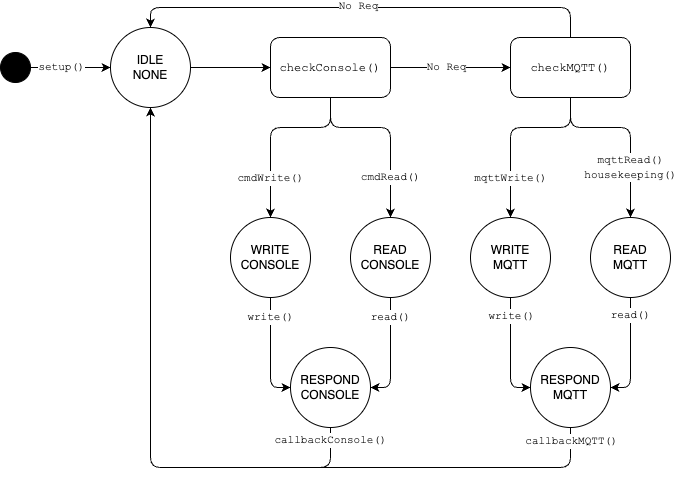
\includegraphics[width=.8\textwidth]{figs/readout/FSM_IF.png}
    \caption[Finite State Machine for the IF Amplifier Control Loop]{Finite State Machine for the IF Amplifier Control Loop. Each state shows the current step in the process followed by the system that requested the action.}
    \label{readout/fig:if_amp_fsm}
\end{figure}

For the Arduino control loop, we have implemented multiple ways to interact with the device using the \texttt{if\_amp} library.
For flight, we will be using the MQTT protocol to send messages to the Arduino to set the attenuation values and read the current attenuation values.
For testing, we have implemented both a simple serial interface. 
A web interface was also developed to control the attenuators using a web browser but was later removed to save on memory. 
Including the web interface adds additional static memory usage to the Arduino Nano Every in the form of large HTML strings.

The structure for the Arduino control loop is a finite state machine that keeps track of the current request and which system requested it.
Figure \ref{readout/fig:if_amp_fsm} shows the state diagram for the finite state machine.

The system starts with \texttt{setup()} which initializes all of the hardware interfaces and sets our initial state to \texttt{IDLE}.
Within \texttt{setup()}, we start our serial interface and initialize the I$^2$C bus.
Because of a hardware issue on the Printed Circuit Board (PCB), the \texttt{Wire} library needs to be patched to include timeouts on the I$^2$C bus.
This is because of a hardware issue where the Arduino has power but the rest of the system is off.
In this scenario, there is a floating voltage on the I$^2$C bus that causes the \texttt{Wire} library to hang indefinitely.
The patched \texttt{Wire} library has a new \texttt{setTimoout()} method that sets a timeout for the I$^2$C bus to prevent this from happening.

After setting up serial and I$^2$C, the system sets up our Ethernet and MQTT connections.
For Ethernet, we are using the W5500 Ethernet shield from Wiznet \parencite{w5500}.
This shield is connected to the Arduino using SPI and enables us to connect the Arduino to the rest of the readout network. 
To setup the networking, we give the Arduino a unique MAC address and a static IP address.
On ASTHROS, we have two of these systems so we provide them with addresses based on their hard coded ID. 
In the case that the Arduino is not connected to the network, the system will continue to run but will only accept messages from the serial interface.
After setting up the Ethernet connection, we setup a client to connect to the MQTT broker.
This client takes the IP address of the broker and the port to connect to and attaches a callback function to handle incoming messages.
We then attempt a connection to the broker through the client using the name of our device and an account on our RabbitMQ server setup for handling MQTT requests.
Once connected, we subscribe to the \texttt{mqtt/comm/<ID>} topic where \texttt{<ID>} is the ID of the Arduino.
While AMQP and MQTT are different protocols, RabbitMQ has a plugin to handle MQTT messages and route them to the correct AMQP exchange.
By default messages published via MQTT are sent to the \texttt{amq.topic} exchange with the MQTT topic as the routing key, replacing the forward slashes with periods.
At the end of \texttt{setup()}, we initialize all of the attenuators to 31.75 dB and set the state to \texttt{IDLE}.

The \texttt{loop()} function is the main function that runs the finite state machine.
On top of the state and system variables, we have array buffers for \texttt{addr}, \texttt{attn}, and \texttt{status} to store the address, attenuation value, and status of the current function call. 
There is also a flag for \texttt{single} that is used to indicate if the current call is for a single channel or all channels.

In the \texttt{IDLE} state, we begin by checking if there is a message available on the serial interface. 
Using the \texttt{StaticSerialCommands} library, we can parse messages and call the appropriate callback function. 
Available commands are \texttt{w <addr> <attn>}, \texttt{wa <attn>}, \texttt{r <addr>}, and \texttt{ra} for writing and reading a single channel or all channels.
These commands do not actually execute the function but instead set the state to \texttt{WRITE} or \texttt{READ} with the appropriate address, attenuation value, and single flag.
We also set the system to \texttt{CONSOLE} to indicate that the serial interface requested the action.
In the case of a single channel operation, the first index of \texttt{addr} and \texttt{attn} are used. 
If the command is not recognized, an error message is sent back to the serial interface and we stay in the \texttt{IDLE} state.

If there are no commands waiting in the buffer and we are connected to the MQTT broker, we check for incoming messages.
If there is a message, we parse the message and set the state to \texttt{WRITE} or \texttt{READ} with the appropriate address, attenuation value, and single flag.
Messages from the MQTT broker are JSON strings with a \texttt{cmd} key that specifies the command and \texttt{addr} and \texttt{attn} keys that specify the address and attenuation value.
Additionally, we record the \texttt{routing\_ID} of the message in order to respond directly to the sender.
MQTT does not support direct addressing so we workaround this by sending a message to the topic exchange with the \texttt{routing\_ID} as the route. 
Whomever sends the request will need to subscribe to the \texttt{mqtt/comm/<routing\_ID>} topic to receive the response.

In the \texttt{READ} state, we call the \texttt{read()} command which begins a read operation on the Arduino. 
\texttt{read()} iterates over either all of the channels or just the first index and calls \texttt{single\_read()}.
The \texttt{single\_read()} function calls the \texttt{set\_attn()} function from the \texttt{if\_amp} library with the address and a pointer to the attenuation value.
We then store the status of the \texttt{set\_attn()} call in the corresponding index of \texttt{status}.
There is an error offset parameter that is used to add an offset to the status in case of errors.
This is used later in \texttt{single\_write()} to differentiate between an error in writing and reading back the value. 
After reading all of the specified channels, we set the state to \texttt{RESPOND}.

In the \texttt{WRITE} state, we call the \texttt{write()} command which begins a write operation on the Arduino.
\texttt{write()} iterates over either all of the channels or just the first index and calls \texttt{single\_write()}.
\texttt{single\_write()} calls the \texttt{set\_attn()} function from the \texttt{if\_amp} library with the address and the attenuation value and saves the status. 
If the status is nonzero, we set the corresponding index in the attenuation buffer to -1 to indicate an error.
If not, we perform a \texttt{single\_read()} with an offset of 100 to indicate any errors in reading back the value came from the read operation. 

After either a read or write operation, the system ends up in the \texttt{RESPOND} state.
In this state, we check the system variable to see who requested the operation.
If the system is \texttt{CONSOLE}, we print out the status, attenuation, and address of either the single channel or all channels.
If the system is \texttt{MQTT}, we package the status, attenuation, and address into a JSON string and publish to the MQTT broker with the \texttt{mqtt/comm/<routing\_ID>} topic.
In either case, after sending the response, we clear the three buffers and set our state back to \texttt{IDLE}.

The firmware also has a few extra features to help configure the system.
The console also accepts an \texttt{mqtt} command that enables or disables the MQTT interface.
This is useful as, if the system is not connected to the network, the MQTT interface will continually try to connect and fail.
At a predefined interval, the system will publish a message to the \texttt{mqtt/comm/<ID>} topic with the status of the system.
This is integrated into our state machine while checking for MQTT message by comparing the last time we published a status message with the current clock time and setting the state to \texttt{READ} and system to \texttt{MQTT} if the time has elapsed.
This read will read all channels and have an additional flag, \texttt{mqttStatus} that is checked in the \texttt{RESPOND} state to publish the status message to the MQTT broker with the \texttt{mqtt/comm/<ID>} topic instead of the routing ID.

There are also some quirks to the system that we attempt to mitigate in the firmware.
In addition to the I$^2$C bus issue, there is a hardware issue where the Ethernet shield will not initialize properly if the IF slices are powered on before the Arduino. 
In this case, we have a \texttt{pulseReset()} function that pulses the reset pin on the Ethernet shield to reset the shield and attempt to initialize the connection.
This occurs because power will leak through the SPI bus and partially power the shield.
When the system is fully on, the shield has an incorrect reference voltage and will not initialize properly during \texttt{setup()}.

\section{Housekeeping}
In our initial implementation of housekeeping, we intended to conform to the structure necessary for downstream processing using GSEOS (Ground Support Equipment Operating System) \parencite{hauck2003use}.
GSEOS is the ground station software previously used by the ASTHROS team to digest and visualize telemetry data from the gondola.
Due to changes on the gondola's software side, the housekeeping system will need to be modified to conform a different framework.
For now, this section will outline the current implementation of the housekeeping system as the connections to the rest of our readout system are still valid. 
Steps for implementing the new system will be outlined in a subsection below.

At it's core, the housekeeping system is the culmination of every other system in the readout pipeline.
Every system previously defined produces some sort of status message that needs to be captured, analyzed, and forwarded to the operations team.
Thanks to all of the groundwork done by \texttt{rmqtools}, we are able to very easily implement a system that can receive messages from every other system on the network and publish them to the GSEOS. 

For the readout system, our route to sending data to GSEOS is a socket open on one of the gondola computers that expects our data in a very specific format such that it can packetize the data and downlink it to the ground station.
Once at the ground station, we are able to take the formatted data and monitor it using the GSEOS software.
Because we have a single pipeline for all of our data, we need to segment and packetize the data into different blocks such that we do not exceed our downlink bandwidth.
To packetize the data properly, we have implemented a \texttt{Housekeeping} library that handles harmonizing data from various subsystems, formatting it for GSEOS, and sending it to the socket at regular intervals. 

At its core, the \texttt{Housekeeping} library is a set of data queues in a fixed sequence, where each data queue is checked in a predefined order on a set interval.
A good analogy for this is a clock, where each position on the clock is a data queue.
When the clock ticks and points to a new position, the data queue at that position is checked for new data.
If there is new data, it is formatted and sent to the socket.
We call these data queues \texttt{blocks}, with each block being unique to the type of data it is processing.

Regardless of the data that is being processed, each block has the following characteristics and behaviors. 
Blocks are setup with a \texttt{msg\_id} signifying the type of data being processed. 
This is used on GSEOS to identify where the data needs to be loaded in the system after it is received.
Following that is \texttt{route} which is a list of all of the RabbitMQ routing keys that this block needs to subscribe to.
Next we have a \texttt{data} class which is a custom \texttt{QueueTTL} object that acts as a dictionary with a time to live (TTL) for each key.
This allows us to consolidate data from multiple sources into a single block without having to worry about sending stale data if one of the sources goes down.
Finally, we have a \texttt{data\_queue} object which is simply a Queue that contains encoded data that is ready to be sent to the socket.

Each block then has a set of methods that are used to handle acquiring and processing the data.
First, the block has a \texttt{subscriber()} method that is structured to be decorated with \texttt{rmqtools} to handle the incoming messages.
As each subsystem may need a different method to handle incoming messages, each block has their own \texttt{subscriber()} method unique to the block's datatype.
Within this method, we retrieve the data, place it in the \texttt{data} object, and then call the \texttt{encode()} method to encode the data for GSEOS before placing it in the \texttt{data\_queue}.
The \texttt{encode()} method is highly dependent on the type of data being processed and is unique to each subsystem, which we will further discuss in subsections for each block. 
At the start of each encoded message is a stamp from \texttt{get\_stamp()}, a utility method that creates a header for the data with a timestamp and the \texttt{msg\_id} of the block.
The end result of the \texttt{encode()} method is a byte array that contains the predefined encoding format for GSEOS.
Finally, we have a \texttt{simulate\_data()} method that is used to simulate data for testing purposes.
This is a counterpart to the \texttt{subscriber()} method as instead of receiving data from RabbitMQ, we generate random data, place it in our \texttt{data} object, and call the \texttt{encode()} method to encode the data for GSEOS.

These blocks handle the logic behind acquiring and encoding data but need to be implemented in the main housekeeping loop.
Before we get to the main loop where our sequenced clock sends data at regular intervals, we need to setup the blocks to receive data. 
This is done by wrapping the \texttt{block.subscriber()} method with \texttt{subscribe\_status} and passing the \texttt{block.route} list to the decorator.
We give these queues the unique name \texttt{housekeeping\_<seq\_id>} where \texttt{<seq\_id>} is the index of the block in the sequence.
When looking at the RabbitMQ console, we are able to easily see which queues are receiving data and which ones are not.
Once all of the blocks are attached to the RabbitMQ server, we can start the listeners and begin the housekeeping loop.
Each listener is on a separate thread and will asynchronously process messages as they come in.
When the housekeeping loop gets to the block's index in the sequence, it will check the \texttt{data\_queue} for any data that is ready to be sent.
In order to get the most recent data, the queue is read until it is empty and the data is sent to the socket.
If there is no data in the queue by the time the clock is ready to move, we skip the block and the loop continues, checking the next block in the sequence for data. 
If there is data, we encode it along with the status of the system and send it to the socket.
Afterwards, we sleep until the next tick of the clock and repeat the process.
In practice, this looks like the following sequence, where the clock has a 12 second cycle and each block is checked every second:
\begin{table}
    \centering
    \begin{tabularx}{\textwidth}{l|l|X}
        \textbf{Timing} & \textbf{Message ID} & \textbf{Block} \\
        \hline
        1 &\texttt{4} & PSU Block for Smart PSU 4 \\
        2 &\texttt{7} & PSU Block for Smart PSU 7 \\
        3 &\texttt{5} & PSU Block for Smart PSU 5 \\
        4 &\texttt{8} & PSU Block for Smart PSU 8 \\
        5 &\texttt{6} & PSU Block for Smart PSU 6 \\
        6 &\texttt{10} & PSU Block for Smart PSU 10 \\
        8 &\texttt{2} & Antenna Block \\
        9 & \texttt{3} & Motor Block \\
        10 & \texttt{1} & Temperature Block \\
        11 & \texttt{11} & Cryocooler Block \\
        12 & \texttt{12} & Intermediate Frequency Block \\
    \end{tabularx}
    \caption{Housekeeping Sequence}
    \label{readout/table:housekeeping_sequence}
\end{table}

\subsection{Antenna Block}
The antenna system is fairly straightforward for implementation.
There is a single \texttt{housekeeping.antenna} routing key to subscribe to and the data is a simple dictionary packed with various readout values from the antenna.
Below is a list of the values that are packed into the data dictionary. 
\begin{itemize}
    \item \texttt{M1\_HW\_VER} - The hardware version of the M1 antenna system.
    \item \texttt{M1\_SW\_VER} - The software version of the M1 antenna system.
    \item \texttt{M2\_HW\_VER} - The hardware version of the M2 antenna system.
    \item \texttt{M2\_SW\_VER} - The software version of the M2 antenna system.
    \item \texttt{M1\_TEMP} - The temperatures of M1's 9 Replicas and their average from -327.68 to 327.67 C. 
    \item \texttt{M2\_TEMP} - The temperatures of M2's 3 Legs, the Leg Average, and the M2 Mirror and Board from -327.68 to 327.67 C.
    \item \texttt{M2\_TEMP\_THRESH} - The lower and upper limits for the thermostat on the M2 from -327.68 to 327.67 C.
    \item \texttt{GPS\_POS} - The Latitude, Longitude, and Altitude of the GPS system from -90 to 90 deg , -180 to 180 deg, and 0 to 428496.7296 m respectively.
    \item \texttt{ELEVATION\_MEAS} - The elevation of the antenna from -90 to 90 deg.
    \item \texttt{HEXA\_POS\_SET} - The current desired position and rotation of the hexapod from -214,748.3648 to 214,748.3647 mm and -214,748.3648 to 214,748.3647 deg respectively.
    \item \texttt{HEXA\_POS\_CORR} - The correction position and rotation of the hexapod from -214,748.3648 to 214,748.3647 mm and -214,748.3648 to 214,748.3647 deg respectively.
    \item \texttt{HEXA\_POS\_REAL} - The actual position and rotation of the hexapod from -214,748.3648 to 214,748.3647 mm and -214,748.3648 to 214,748.3647 deg respectively.
    \item \texttt{FLAGS} - Status enabled flags from the M1 and M2 Heaters, the M2 thermostat, and the Hexapod correction. 
    \item \texttt{ALARMS} - Status alarms indicating issues communicating with the M2 or Hexapod controllers, the legs being too cold from the M2 thermostat, or a bad elevation reading.
\end{itemize}

\subsection{Cryocooler Block}
The cryocooler block is similar to the antenna block in that it is a simple dictionary of values from the cryocooler system.
Unlike the antenna block, the cryocooler block has three routes to listen to, \texttt{housekeeping.cryo}, \texttt{housekeeping.lakeshore.cal}, and \texttt{housekeeping.lakeshore.temp}.
Within the \texttt{subscriber()} method, we check the routing key of the incoming message and handled each one accordingly. 
Because our \texttt{QueueTTL} object handles the TTL of each key, we simply \texttt{put()} the data into the \texttt{data} object and the logic for handling stale data is handled when we call \texttt{get()}. 

As for the data, the cryocooler provides these values as bytes so all we need to do is ensure the data is in the right order and then pass the bytes to the \texttt{data\_queue}. 
This results in minimal processing for the data from \texttt{housekeeping.cryo} but we will still need to process the data from \texttt{housekeeping.lakeshore.cal} and \texttt{housekeeping.lakeshore.temp} as they are not in the correct format for GSEOS.
Below is the complete list of values that are packed into the data dictionary for the cryocooler block.
\begin{itemize}
    \item \texttt{status} - The current status byte of the cryocooler.
    \item \texttt{caseTemp} - The temperature of the case.
    \item \texttt{reserve} - Reserved value (typically not used).
    \item \texttt{piOut} - Voltage output of the PI Loop.
    \item \texttt{busVoltPeak} - Bus voltage at the motor voltage peak.
    \item \texttt{controlTemp} - The temperature of the control sensor.
    \item \texttt{auxTemp} - The temperature of the auxiliary sensor.
    \item \texttt{busCurr} - The current of the bus.
    \item \texttt{busVoltAvg} - The average voltage of the bus.
    \item \texttt{opMode} - The current operating mode.
    \item \texttt{compFreq} - The frequency of the compressor motor.
    \item \texttt{tempSet} - The desired temperature for Cold Head 1.
    \item \texttt{motorDrive} - The peak output of the voltage drive.
    \item \texttt{intGain} - The integral factor of the PI temperature and voltage controller.
    \item \texttt{propGain} - The proportional factor of the PI temperature and voltage controller.
    \item \texttt{peakDrive} - The voltage limit on the peak output of the bus.
    \item \texttt{motorPeakPos} - The peak positive voltage of the motor.
    \item \texttt{motorPeakNeg} - The peak negative voltage of the motor.
    \item \texttt{avcPeakPos} - The peak positive voltage of the AVC (Adaptive Vibration Control).
    \item \texttt{avcPeakNeg} - The peak negative voltage of the AVC.
    \item \texttt{voltRamp} - The maximum voltage ramp rate.
    \item \texttt{lsCal} - The calibration temperatures (2) of the Lakeshore, encoded as data from 0 to 65535 to be later converted to a float
    \item \texttt{lsCryo} - The cryocooler temperatures (8) of the Lakeshore from 0 to 65,535.99 K. 
\end{itemize}

\subsection{Intermediate Frequency Block}
The IF block is one of the more simple blocks in the system.
Unlike the other systems, the IF systems does not use the traditional \texttt{status} exchange as it operates using the MQTT protocol. 
Our RabbitMQ server has a plugin to handle MQTT messages and route them to the \texttt{amq.topic} exchange. 
As such, we have a separate \texttt{RmqConnection} object whose status exchange is set to \texttt{amq.topic} and use this object to wrap the block's \texttt{subscriber()} method.
For routing, we subscribe to \texttt{mqtt.status.0}, \texttt{mqtt.status.1} and \texttt{mqtt.status.2} for the three IF slices.
Each slice has up to 8 channels, except for slice 0 which only has 1 for the 100GHz receiver. 
This is a total of 17 channels that we need to monitor.
The data from the IF block is a simple dictionary of attenuation values in dB as well as the status flag from each channel.
We pack this data into a byte array, consisting of all of the attenuation values followed by the status flags.

\subsection{Motor Block}
The motor block is another relatively simple system.
The motor only has one route, \texttt{housekeeping.motor}, which receives the mirror position from the motor controller.
The following values are packed into the byte array for the motor block.
\begin{itemize}
    \item \texttt{HC} - Hold Current as a percentage of the maximum current\footnote{\label{readout/footnote:motor}This value is a user set value and should not change during operations. We downlink this value in case it does change due to an error in the system.}
    \item \texttt{RC}- current as a percentage of the maximum current$^{\ref{readout/footnote:motor}}$
    \item \texttt{A} - The acceleration of the motor in steps per second squared$^{\ref{readout/footnote:motor}}$.
    \item \texttt{D} - The deceleration in steps per second squared$^{\ref{readout/footnote:motor}}$.
    \item \texttt{VM} - The maximum velocity of the motor in steps per second$^{\ref{readout/footnote:motor}}$.
    \item \texttt{VI} - The initial velocity in steps per second$^{\ref{readout/footnote:motor}}$.
    \item \texttt{P} - The current position of the motor in steps.
    \item \texttt{CB} - The current control bounds, a mode selection for torque performance$^{\ref{readout/footnote:motor}}$.
    \item \texttt{ER} - The error code from the motor controller.
\end{itemize}

\subsection{Smart PSU Block}
The Smart PSU block is one of the more densely packed blocks in the system.
Because we have so many Smart PSUs, we actually have multiple \texttt{PsuBlock} objects in the sequencer so that we can have separate threads for each PSU and spread out the bandwidth to the GSEOS socket.
The route for each of these blocks is variable and set to \texttt{housekeeping.psu.<psu\_id>} where \texttt{<psu\_id>} is the ID of the PSU, which is also the \texttt{msg\_id} for the block. 
The actual data from the Smart PSUs are the voltages, currents, and enabled status from each channel as well as some overhead data for the PSU itself.
The data is packed into a byte array with the following values:
\begin{itemize}
    \item \texttt{A\_Voltage} - The voltage from bank A, channels 0 to 7, from -32.76 to 32.76 V.
    \item \texttt{B\_Voltage} - The voltage from bank B, channels 0 to 3, from -32.76 to 32.76 V.
    \item \texttt{C\_Voltage} - The voltage from bank C, channels 0 to 4, from -32.76 to 32.76 V.
    \item \texttt{D\_Voltage} - The voltage from bank D, channels 0 to 3, from -32.76 to 32.76 V.
    \item \texttt{E\_Voltage} - The voltage from bank E, channels 0 to 7, from -32.76 to 32.767 V.
    \item \texttt{S\_Voltage} - The voltage from bank S (the synthesizer), channels 0 and 1, from -32.76 to 32.76 V.
    \item \texttt{A\_Current} - The current from bank A, channels 0 to 7, from -99.99 to 99.99 A.
    \item \texttt{B\_Current} - The current from bank B, channels 0 to 3, from -99.99 to 99.99 A.
    \item \texttt{C\_Current} - The current from bank C, channels 0 to 4, from -99.99 to 99.99 A.
    \item \texttt{D\_Current} - The current from bank D, channels 0 to 3, from -99.99 to 99.99 A. This value is actually read from the voltage of the X bank divided by a scaling factor. 
    \item \texttt{E\_Current} - The current from bank E, channels 0 to 7, from -99.99 to 99.99 A.
    \item \texttt{S\_Current} - The current from bank S (the synthesizer), channels 0 and 1, from -99.99 to 99.99 A.
    \item \texttt{Enabled} - The status of each channel as a big endian bit array with each bit representing the status of a channel for banks A, B, C, D, E, and S.
    \item \texttt{Synth\_ID} - The ID of the synthesizer, should be "MLVS-1520AS" and is downlinked for verification we have an SPI connection.
    \item \texttt{Synth\_Freq} - The frequency of the synthesizer in MHz, from 0 to 99999.99 MHz.
    \item \texttt{Synth\_Temp} - The internal temperature of the synthesizer in C, from -327.68 to 327.67 C.
    \item \texttt{Synth\_Max\_Temp} - The maximum temperature of the synthesizer in C, from -327.68 to 327.67 C.
    \item \texttt{Synth\_Status} - The status code from the system, a bit array with each bit representing a different status flag. This value is actually 9 bits long so we zero pad the value to 16 bits.
    \item \texttt{Error\_Codes} - 4 bit error codes for each channel indicating: OK, Voltage Low, Voltage High, Current Low, Current High, Out of Tolerance, and Channel enabled/disabled when expected to be disabled/enabled.
\end{itemize}
\subsection{Temperature Block}
The temperature block also interacts with the Smart PSU system but is focused on the temperature sensors attached to each PSU.
We don't need to split the temperature block into multiple blocks as we're able to fit all of our combined data into a single block.
For routing, we have 6 routing keys for the 6 power supplies on the gondola, \texttt{housekeeping.temp.<psu\_id>} where \texttt{<psu\_id>} is the ID of the PSU.
Apart from that, the rest of the block is very simple. 
We load in a configuration file that contains a mapping of every temperature sensor's ID and a description of the sensor's location. 
We use the ordering of this configuration file to determine the order of the sensors in the data array.
Other than that, we simply iterate over the sensors in the configuration file and use the ID as a key in the \texttt{data} object to order and encode each value from -327.68 to 327.67 C.

\section{Central Command}
The core of the entire readout network is the central command system.
In developing the central command system, we had two goals in mind: develop something that was easily adaptable to whatever subsystems we needed to control and develop something that whose interface would be identical in both testing and in flight.
This led us to looking towards \texttt{click}, a Python library for building command line applications \parencite{click}.
Click enabled us to create a custom command line interface (CLI) that consolidated all of our systems into a single interface.
Additionally, with \texttt{click\_repl}, we were able to create a read-eval-print loop (REPL) that would act as a terminal interface to the system, allowing us to chain commands together and interact with the system in a more natural way.

To accomplish the first of these two goals, we utilize click's ability to add groups and subcommands to the CLI.
We call these \texttt{plugins} and simply developed a plugin for each subsystem that we needed to control. 
Separating each of the subsystems into their own plugins allow us to easily develop new plugins for new subsystems without having to modify the core of the system.
At the core of each plugin is a unique \texttt{Controller}, which handles methods necessary for interacting with the subsystem in the plugin.
Usually, this interaction with the subsystem is done through a RabbitMQ connection, sending RPC executions to the subsystem and waiting for a response.
Normally, each command sent is atomic, where each command's execution exists in a vacuum, but we can work around this by storing a persistent \texttt{Controller} in within \texttt{click.get\_current\_context()}. 
This allows us to store the state of the system between commands, create global variables that are accessible to all commands, and, most importantly, only need to create a single instance of the \texttt{Controller} for each plugin.

In terminal mode, we are able to accomplish our second goal of having a single interface for both testing and flight.
Terminal mode is a special mode of the CLI that uses a REPL to allow the user to interact with the system in a more natural way, without having to type out \texttt{python central\_command.py --config config.yml ...} every time.
Within terminal mode, the first thing you type is the name of the plugin you want to interact with, which loads the plugin and gives you access to all of the commands in that plugin.
It also has tab completion for all of the commands in the plugin, so you can easily see what commands are available.
There is additionally a history feature that allows you to scroll through the previous commands you have entered, and use reverse search to find commands you have entered in the past.
We primarily use this terminal interface for testing, as it allows us to easily interact with the system in an isolated environment.
To match the flight system, we have implemented a version of Central Command that listens to a socket and receives strings from the ACE computer on the gondola. 
The string is then parsed exactly as it would be in the terminal interface, and the command is executed as if it were entered in the terminal, making it identical to the REPL system when in flight. 
The biggest challenge here is capturing the output of the command and sending it back to the ACE computer.
This is done by exclusively using the \texttt{click.echo()} method to print to the terminal in REPL mode and then overriding the behavior of \texttt{click.echo()} to send the output to the socket instead of printing it to the terminal.

\begin{table}
    \centering
    \begin{tabularx}{\textwidth}{l|X}
        \textbf{Plugin} & \textbf{Description} \\
        \hline
        \texttt{antenna} & Controls the Antenna Systems. \\
        \texttt{cryo} & Controls the Cryocooler Systems. \\
        \texttt{fabric} & An implementation of the \texttt{fabric} allowing us to execute commands on any computer on the network in case of emergency. \\
        \texttt{ifsys} & Controls the Intermediate Frequency Systems. \\
        \texttt{motor} & Controls the Mirror's Motor Systems. \\
        \texttt{pressure} & Controls the Pressure Systems. \\
        \texttt{psu} & Controls the Smart PSU Systems. \\
        \texttt{seq} & A special system that allows us to execute commands in a sequence, similar to a script. \\
        \texttt{spec} & Controls the Spectrometer Systems. \\
        \texttt{synth} & Controls the Synthesizer Systems. \\
    \end{tabularx}
    \caption{Plugins for the Central Command System}
    \label{readout/table:click_plugins}
\end{table}

Table \ref{readout/table:click_plugins} shows a list of the plugins that are currently implemented or planned for the system.
Two plugins do not control a specific subsystem but are instead used to provide broad functionality to ASTHROS.
\texttt{seq} is a special scripting plugin that allows us to write a sequence of commands to be executed in order as a text file. 
When the file is executed, it is parsed and each command is executed in order.
This makes running a sequence of commands, such as starting up the spectrometer, or running a test sequence, much easier.
For flight, we will develop sequences for most operations that need to be performed as it allows us to reduce our required bandwidth to the ground station when issuing multiple commands. 
Likewise, the \texttt{fabric} plugin is a special plugin that allows us to execute commands on any computer on the network.
\texttt{fabric} is a Python library that allows us to execute commands on remote computers over SSH. 
While we would hope that our Central Command system is able to handle all required commands, there may be times when we need to execute a raw command on a remote computer.
This is especially useful in flight, when SSHing into a computer may not be possible and we need a backup plan.

For the spectrometer system, we had to handle multiple instances of subsystems responding to the same command.
This occurs as we have multiple CM4s on the gondola, each with their own spectrometer system.
To handle this, we place a \texttt{PriorityLock} on the response handler for the command so that only one command is executed at a time.
Each command updates a response dictionary with the response from the command, which harmonizes the responses into a single dictionary.
This allows us the end user to transparently communicate with multiple spectrometer systems at once without having to worry about the underlying implementation.

\section{Future Work}
\label{readout/section:future}
One of the final steps in the readout system is to implement the functionality for on-board analysis and anomaly detection.
When the spectrometers finish an HDF5 file, it is flagged in the ODOO database for processing.
Currently, we have scripts built out that take the timestamps from the HDF5 file and harmonize them with data queried from the ODOO database from that time period.
The data is then interpolated and processed to create a Level 1 data product that can be used for analysis.
A single test was done before ASTHROS was packed up generating a Level 1 data product from the HDF5 file and the ODOO database.
The results were promising, but due to an error in how we stored the timestamps in the HDF5 file, we were unable to properly align the data with the temporal precision necessary for map making.
With further testing of the readout system and the gondola system, we will be able to refine the process and ensure that the data is properly aligned for analysis.

For Level 2 data products, we plan to chop and smooth the data to reduce the overall size of the files for downlinking and analysis. 
We are still working on discussing appropriate signal to noise ratios (SNR) for the snapshot data products, but methods to perform this are already implemented. 
Both the Level 1 and Level 2 data product prototypes have been created but not fully implemented in the readout system as an automated process on the Analysis computer. 
The Level 2 data would then be downlinked to the ground station for further analysis and archiving.
This allows us to create maps while the flight is still ongoing, allowing us to quickly identify any issues with the data and make adjustments as necessary.

Another feature for the Analysis computer is to implement a system that can detect anomalies in the data.
The theory behind our approach is outlined in \ref{ch:spectra} but we have not yet implemented the system in the readout pipeline.
The information we receive from the gondola is not sufficient in determining which spectra are ON and OFF measurements, so work will need to be done in conjunction with the gondola systems team to ensure we have the necessary information to perform the anomaly detection.
We could, in theory, perform the anomaly detection on every spectra, regardless of whether it is an ON or OFF measurement, but this would result in a lot of false positives and would not be useful for mission operations.
Calculating just on the OFF measurements would produce anomaly scores that are the most useful for mission operations as these calibration measurements will likely be the most stable as they are not dependent on the target being observed.

In addition to analysis steps, there are calibration tasks left to be done with the PMCCs.
Currently, we are using the manufacturer suggested default settings for the spectrometers and they perform well for most of our science goals.
However, if we were to read out these spectrometers at a much faster rate, it would unlock new ways for us to collect data and help our overall commissioning after launch.
We can achieve these data rates by limiting the number of channels in the spectrometer to integrate at a lower spectral resolution but with a higher temporal bandwidth. 
Because of how we designed the \texttt{PyMCC} module, these changes can be easily made in the configuration file for both testing and generation of mode specific configs.

Finally, there is a good deal of polishing that needs to be done once all of the readout systems are implemented with the gondola systems.
The two systems were developed with an agreed upon interface but there are still some discrepancies that need to be resolved.
Given the changes to the gondola, we may be starting from scratch with the gondola systems team, but the readout system will remain the same.
This actually gives us more flexibility in how we integrate the readout system with the gondola system as we can have more control over the interface and between the two systems.